\documentclass[pdflatex,11pt]{aghdpl}
% \documentclass{aghdpl}               % przy kompilacji programem latex
% \documentclass[pdflatex,en]{aghdpl}  % praca w języku angielskim
\usepackage[polish]{babel}
\usepackage[utf8]{inputenc}

% dodatkowe pakiety
\usepackage{enumerate}
\usepackage{listings}
\usepackage{color}
\definecolor{lightgray}{rgb}{.96,.96,.96}
\definecolor{darkgray}{rgb}{.4,.4,.4}
\definecolor{purple}{rgb}{0.65, 0.12, 0.82}

\lstloadlanguages{TeX}

\lstset{
  literate={ą}{{\k{a}}}1
           {ć}{{\'c}}1
           {ę}{{\k{e}}}1
           {ó}{{\'o}}1
           {ń}{{\'n}}1
           {ł}{{\l{}}}1
           {ś}{{\'s}}1
           {ź}{{\'z}}1
           {ż}{{\.z}}1
           {Ą}{{\k{A}}}1
           {Ć}{{\'C}}1
           {Ę}{{\k{E}}}1
           {Ó}{{\'O}}1
           {Ń}{{\'N}}1
           {Ł}{{\L{}}}1
           {Ś}{{\'S}}1
           {Ź}{{\'Z}}1
           {Ż}{{\.Z}}1
}

\lstdefinelanguage{JavaScript}{
  keywords={typeof, new, true, false, catch, function, return, null, catch, switch, var, if, in, while, do, else, case, break},
  keywordstyle=\color{blue}\bfseries,
  ndkeywords={class, export, boolean, throw, implements, import, this},
  ndkeywordstyle=\color{darkgray}\bfseries,
  identifierstyle=\color{black},
  sensitive=false,
  comment=[l]{//},
  morecomment=[s]{/*}{*/},
  commentstyle=\color{purple}\ttfamily,
  stringstyle=\color{red}\ttfamily,
  morestring=[b]',
  morestring=[b]"
}

\lstset{
   language=JavaScript,
   backgroundcolor=\color{lightgray},
   extendedchars=true,
   basicstyle=\footnotesize\ttfamily,
   showstringspaces=false,
   showspaces=false,
   numbers=left,
   numberstyle=\footnotesize,
   numbersep=9pt,
   tabsize=4,
   breaklines=true,
   showtabs=false,
   captionpos=b
}
%---------------------------------------------------------------------------

\author{Piotr Janik}
\shortauthor{P. Janik}

\titlePL{Wydajna symulacja dynamiki płynów i~przewodnictwa cieplnego w~środowisku przeglądarki internetowej}
\titleEN{Efficient Simulation of Fluid Dynamics and Heat Transfer in~the~Web~Browser Environment}

\shorttitlePL{Wydajna symulacja dynamiki płynów i przewodnictwa cieplnego w przeglądarce internetowej} % skrócona wersja tytułu jeśli jest bardzo długi
\shorttitleEN{Efficient Simulation of Fluid Dynamics and Heat Transfer in the Web Browser Environment}

\thesistypePL{Praca magisterska}
\thesistypeEN{Master of Science Thesis}

\supervisorPL{prof. dr hab. inż. Witold Dzwinel}
\supervisorEN{Witold Dzwinel, Prof.}

\date{2012}

\departmentPL{Katedra Informatyki}
\departmentEN{Department of Computer Science}

\facultyPL{Wydział Elektrotechniki, Automatyki, Informatyki i Elektroniki}
\facultyEN{Faculty of Electrical Engineering, Automatics, Computer Science and Electronics}

\acknowledgements{Serdecznie dziękuję \dots}



\setlength{\cftsecnumwidth}{10mm}

%---------------------------------------------------------------------------

\begin{document}

\titlepages

\begin{abstract}

Celem niniejszej pracy było stworzenie wydajnej symulacji dynamiki płynów oraz
przewodnictwa cieplnego działającej w środowisku przeglądarki internetowej.
Aplikacja ma charakter edukacyjny, a jej głównym zadaniem jest wspieranie
użytkownika w dogłębnym zrozumieniu procesu transferu energii, w tym zjawisk
takich jak przewodnictwo cieplne, konwekcja czy różnorodne przepływy gazów i
cieczy. Projekt został zrealizowany przy współpracy \mbox{z The Concord
Consortium}, amerykańską organizacją \mbox{non-profit} zajmującą się wspieraniem
edukacji poprzez technologię.

Implementacja symulatora w przeglądarce internetowej była niezwykle istotna ze
względu na jego edukacyjne zastosowanie -- kluczowym wymaganiem była dostępność
dla jak najszerszego grona użytkowników, przenośność, wieloplatformowość oraz
możliwość łatwego osadzania w wirtualnych podręcznikach szkolnych nowej
generacji. Z drugiej strony, o jakości symulacji fizycznej w dużej mierze
decyduje jej wydajność czyli efektywne wykorzystanie zasobów. Do niedawna stało
to w sprzeczności z implementacją w języku \emph{JavaScript} oraz wykonywaniem w
środowisku przeglądarki internetowej. 
 
Realizacja tych pozornie wykluczających się wymagań została osiągnięta dzięki
implementacji uwzględniającej budowę i ograniczenia silników \emph{JavaScript} w
nowoczesnych przeglądarkach oraz dzięki przeniesieniu większości obliczeń na
procesor karty graficznej wykorzystując technologię \emph{WebGL}. Jest to
podejście nowatorskie, gdyż dopiero wraz z niedawnym rozpowszechnieniem się
standardu \emph{HTML5} zasoby kart graficznych stały się dostępne dla aplikacji
internetowych w tak szerokim zakresie.

W pracy zostały przedstawione najważniejsze, nowoczesne techniki umożliwiające
tworzenie wydajnych, równoległych aplikacji działających w przeglądarce
internetowej z wykorzystaniem języka \emph{JavaScript} oraz technologii
\emph{WebGL}. Szczegółowo zostały również opracowanie rezultaty oraz korzyści
płynące ze zrównoleglenia symulacji fizycznej. W efekcie powstał wydajny
symulator, który dzięki swojej dostępności oraz jakości może mieć niezwykle
szeroki wpływ na edukację i zrozumienie fizyki przez użytkowników na różnych
etapach procesu kształcenia.

\end{abstract}


\tableofcontents
\clearpage

\chapter{Wprowadzenie}
	\section{Motywacja}
	\section{Cel pracy}
	\section{Organizacja dokumentu}

\chapter{Wprowadzenie}
\label{cha:wprowadzenie}

Większość ludzi w swoich domach i pracy może korzystać z dorobku technologicznej
rewolucji, która miała miejsce w ostatnich latach. Jednak w niektórych
dziedzinach życia zmiany następują znacznie wolniej - jedną z nich jest
edukacja. Komputery i internet stały się dostępne w większości szkół, jednak
programy i metody nauczania często nie nadążają za postępem technologicznym, są
wciąż reliktem poprzedniej epoki. Uczniowie pracują na komputerach najnowszej
generacji, jednak zwykle wykorzystują tylko ułamki ich możliwości, nie mając
dostępu do narzędzi, które faktycznie mogłyby przyczynić się do lepszego
zrozumienia poruszanych na lekcjach zagadnień. Najczęściej komputer i internet
stają się po prostu źródłem łatwo dostępnej wiedzy czy też miejscem gdzie pewne
problemy można próbować rozwiązywać wspólnie. Jest to oczywiście prawidłowe i
wartościowe wykorzystanie nowoczesnej technologi, ale jednocześnie też dosyć
powierzchowne i niewyczerpujące jej pełnych możliwości. Problemy i wyzwania
stojące przed współczesną edukacją szerzej porusza Andrew A. Zucker
\cite{Zuc2009}.

Edukacja może skorzystać na technologicznej rewolucji w znacznie większym
stopniu - jednym z pomysłów są wirtualne laboratoria, które pozwolą uczniom
eksplorować wybrane zagadnienia w sposób interaktywny, szczególnie podczas
nauczania przedmiotów ścisłych i przyrodniczych, tak istotnych w dzisiejszych
czasach. Cyfryzacja powinna zmienić tradycyjne oblicze lekcji z podręcznikiem i
zeszytem na pracę przy narzędziach edukacyjnych nowej generacji, wykorzystując
powszechną dostępność nowoczesnych technologii. Takie aplikacje również
doskonale wpisują się w popularną ideę cyfrowych podręczników. Dosłowne
przeniesienie zawartości papierowych książek na ekrany komputerów nie wiązałoby
się ze znaczącymi zmianami - inny byłby tylko nośnik słów, wiedzy. Bez zmian
natomiast pozostałby sam proces i metody uczenia przez uczniów i studentów.
Jednak jeśli wirtualny podręcznik zostanie zintegrowany z interaktywnymi
aplikacjami, pozwoli to zupełnie zmienić oblicze nauki. Uczeń będzie miał
możliwość prawdziwej eksploracji zagadnień, eksperymentowania we własnym domu,
przed własnym komputerem, podczas codziennej nauki, która może zamienić się w
prawdziwą, wartościową i przede wszystkim rozwijającą przygodę.

Najlepszym pomysłem dla podręczników przyszłości wydaje się umiejscowienie ich w
internecie. Dzięki dystrybucji poprzez to medium można uzyskać niezwykle łatwy i
powszechny dostęp, jako że połączenie z internetem jest w dzisiejszych czasach
czymś w pełni osiągalnym. Internetowa dystrybucja niesie również mnóstwo
korzyści nie tylko dla użytkowników podręczników, ale także dla ich twórców -
wystarczy wymienić zalety takie jak łatwość aktualizacji i docierania do
odbiorców. W związku z tym, również narzędzia stanowiące interaktywne elementy
podręczników przyszłości powinny być przystosowane do działania w środowisku
przeglądarki internetowej. Jest to zadanie wymagające, jednak niedawny rozwój
technologii i standardów internetowych takich jak HTML5 oraz WebGL, jak również
gwałtowne zmiany w samych przeglądarkach internetowych, dają ogromne możliwości
w tej materii.

Wymienione pomysły nie są tylko planami na przyszłość - te zmiany już powoli
następują, cyfrowe podręczniki i wirtualne laboratoria są trakcie rozwoju. Jedną
z organizacji zajmujących się wprowadzaniem najnowszych osiągnięć techniki do
szkół jest \mbox{The Concord Consortium}.

\section{Cel pracy}
\label{sec:celPracy}

W wyniku współpracy ze wspomnianą organizacją \mbox{The Concord Consortium}
powstał wydajny symulator fizyczny prezentujący zjawisko przewodnictwa cieplnego
oraz dynamikę płynów działający w środowisku przeglądarki internetowej o nazwie
\emph{\mbox{Energy2D}}. Ta interaktywna aplikacja doskonale wpisuje się w
przedstawioną ideę wirtualnych podręczników i laboratoriów, umożliwiając
użytkownikom łatwiejsze zrozumienie praw fizyki, które rządzą transferem
energii.

Celem niniejszej pracy jest przedstawienie rozwiązań, które umożliwiły powstanie
symulatora, ze szczególnym naciskiem na technologię WebGL, której niestandardowe
i nowatorskie zastosowanie pozwoliło zrównoleglić obliczenia fizyczne i tym
samym osiągnąć znaczący wzrost wydajności.

\section{Organizacja dokumentu}
\label{sec:organizacjaDokumentu}

Dalsze rozdziały przedstawiają kolejno:

\begin{itemize} \item Przedstawienie możliwości symulatora \en, wprowadzenie
do problematyki symulacji dynamiki płynów i przewodnictwa cieplnego oraz
przegląd istniejących, podobnych rozwiązań.

\item Opis podstawowej implementacji aplikacji, ze szczególnym uwzględnieniem
zagadnień związanych z jej architekturą i wnioskami, które można rozszerzyć na
ogół złożonych systemów \ow{JavaScript}.

\item Prezentację kluczowych technik dzięki którym udało się zrównoleglić
silniki fizyczne symulatora \en przy pomocy technologii \ow{WebGL}.

\item Ocenę systemu, w szczególności testy jakościowe, wydajnościowe oraz
badanie jak konfiguracja sprzętowa użytkownika wpływa na odbiór i jakość
symulacji.

\item Podsumowanie, wnioski, oraz pomysły na dalszy rozwój aplikacji.
\end{itemize}
	
	
\chapter{Symulacja dynamiki płynów i przewodnictwa cieplnego jako wartościowe narzędzie edukacyjne}
	\section{Zastosowanie oraz wpływ na edukację}
	\section{Motywacja i uzasadnienie osadzenia symulacji w środowisku przeglądarki internetowej}
	\section{Zastosowane silniki fizyczne}
		\subsection{Równanie Naviera-Stokesa}
		\subsection{Równanie przewodnictwa cieplnego}
	\section{Zjawiska modelowane przez symulator}
		\subsection{Transfer ciepła}
			\subsubsection{Przewodnictwo cieplne}
			\subsubsection{Konwekcja}
		\subsection{Przepływ płynów}
			\subsubsection{Przepływ laminarny}
			\subsubsection{Przepływ turbulentny}
	\section{Dostępne, istniejące rozwiązania}
		\subsection{Przegląd}
		\subsection{Prekursor systemu - aplikacja Energy2D}


\chapter{Problematyka tworzenia złożonych systemów w języku JavaScript}
	\section{Główne braki środowiska JavaScript w kontekście złożonych systemów}
	
	\section{Technologie przełamujące ograniczenia JavaScript}
		\subsection{Nowoczesne przeglądarki internetowe oraz rozwój interpreterów JavaScript}
			\subsubsection{Chromium V8}
		\subsection{HTML5}
		\subsection{WebGL}
		\subsection{Specyfikacja CommonJS}
		\subsection{Node.js jako zaawansowany interpreter JavaScript oderwany od przeglądarki}
			\subsubsection{Przegląd możliwości}
			\subsubsection{Schemat tworzenia aplikacji działającej zarówno w przeglądarce jak i
							środowisku Node.js}
									
	\section{Techniki zrównoleglania aplikacji JavaScript}
		\subsection{Typowe metody, a przeglądarka internetowa}
		\subsection{WebGL -- otwarcie dostępu do zasobów karty graficznej}
		\subsection{Niskopoziomowe przenoszenie obliczeń na procesor karty graficznej}		

\chapter{Implementacja symulatora w środowisku przeglądarki internetowej}
	\section{Architektura - wzorzec Model-View-Controller}
	\section{Zgodność ze środowiskiem Node.js oraz przeglądarką internetową}
	\section{Przegląd najistotniejszych jednostek symulatora}
	\section{Optymalizacje pod kątem współczesnych interpreterów JavaScript}

\chapter{Przeniesienie obliczeń fizycznych na procesor karty graficznej}

Niniejszy rozdział prezentuje techniki zastosowane w celu przeniesienia głównych
obliczeń fizycznych na kartę graficzną w symulatorze \ow{Energy2D} będącym
przedmiotem tej pracy. Na początku opisane są tradycyjne podejścia do tego
problemu dla aplikacji działających w natywnym środowisku systemu operacyjnego
oraz ich odniesienie do środowiska oferowanego przez przeglądarki internetowe.
Następnie zaprezentowane zostały najważniejsze zagadnienia dotyczące
implementacji równoległych silników fizycznych \ow{Energy2D} działających na
procesorze karty graficznej. Informacje te mogą być szczególnie użyteczne przy
próbach podobnych optymalizacji innych aplikacji.

Dzięki przeniesieniu obliczeń fizycznych na GPU uzyskano istotny wzrost
wydajności. Dokładna analiza zysków ze zrównoleglenia symulacji jest przedstawiona
w rozdziale \ref{cha:ocena}.

\section{Typowe metody przenoszenia obliczeń na GPU, a przeglądarka internetowa}

Współczesna karty graficzne posiadają ogromną moc obliczeniową -- wielokrotnie
większą od centralnego procesora przy założeniu, że obliczenia da się wykonywać
w sposób równoległy. Pomysł aby przenieść część obliczeń ogólnego zastosowania
na kartę graficzną pojawił się wraz z dynamicznym rozwojem procesorów
graficznych. Szczególnie istotnym momentem było wprowadzenie programowalnych
jednostek cieniujących (specyfikacja \ow{DirectX 8}). Dalszy rozwój obliczeń
ogólnego zastosowania na kartach graficznych (ang. \emph{General-Purpose
Computing on Graphics Processing Units}, w skrócie GPGPU) miał miejsce wraz z
wprowadzeniem technologii, które ukryły złożoność dostępu do zasobów karty
graficznej i udostępniły interfejs wysokiego poziomu. Wiodącymi technologiami
tego typu są \ow{OpenCL} (rozwiązanie otwarte) oraz \ow{CUDA} (zamknięte
rozwiązanie firmy NVIDIA, działające wyłącznie na sprzęcie tego producenta).

Wspomniane powyżej technologie dotyczą oczywiście aplikacji pisanych w natywnym
środowisku systemu operacyjnego. Aby programować jednostki cieniujące wystarczy
podstawowy dostęp do standardowego interfejsu \ow{OpenGL} bądź \ow{Direct3D}.
Implementacje tych interfejsów można znaleźć dla prawie każdego współczesnego
języka programowania. Interfejsy wyższego poziomu (\ow{OpenCL}, \ow{CUDA})
również posiadają implementacje w różnych językach programowania, choć
najczęstszym środowiskiem ich działania są aplikacje napisane w C bądź C++.

Poniżej krótko przedstawione są sposoby przeprowadzania obliczeń ogólnego
zastosowania na kartach graficznych oraz ich związek ze specyficznym
środowiskiem przeglądarki internetowej.

\subsection{Niskopoziomowe programowanie jednostek cieniujących}
\label{subsec:niskProgJedn}

Jest to najstarsze podejście do przeprowadzania obliczeń ogólnego zastosowania
na procesorze karty graficznej. Programista w swoisty sposób ,,oszukuje'' kartę
graficzną, przeprowadzając renderowanie prostej geometrii wyłącznie w celu
uruchomienia własnych programów jednostek cieniujących, które wykonują
obliczenia często nie mające nic wspólnego z generowaniem obrazu.

W przypadku technologii \ow{WebGL}, która posłużyła do zaimplementowania
silników fizycznych \en, diagram potoku renderowania prezentuje rysunek
\ref{fig:WebGLPipeline}. Zielonym kolorem zostały oznaczone procesy, które są
programowalne. Są to dwa rodzaje programów jednostek cieniujących --
wierzchołków oraz fragmentów. Nie ma możliwości bezpośredniego sterowania
pozostałymi procesami. Odbywają się one automatycznie, ewentualnie możliwa jest
konfiguracja pewnych parametrów. Dlatego też cały algorytm przeznaczony do
zrównoleglenia musi zostać zapisany wyłącznie przy użyciu programów wierzchołków
oraz fragmentów. Ponadto dane powinny się znajdować w pamięci karty graficznej,
najczęściej w postaci dwuwymiarowych tekstur.

\begin{figure}[!h]
\centering
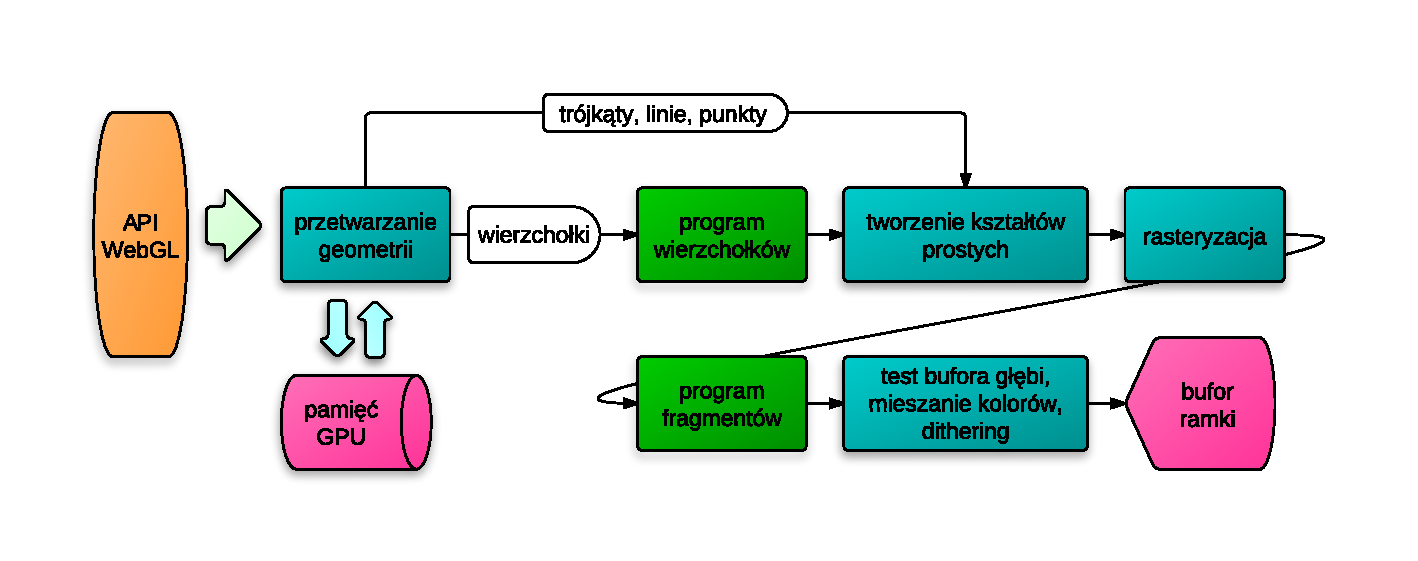
\includegraphics[width=\textwidth]{img/WebGLPipeline}
\caption{Diagram potoku renderowania \ow{WebGL} / \ow{OpenGL 3.x}}
\label{fig:WebGLPipeline}
\end{figure}

Takie podejście jednak jest wymagające i obarczone pewnymi problemami. Łatwo
popełnić błędy, wymagana jest też przynajmniej podstawowa wiedza o programowaniu
grafiki trójwymiarowej. Najważniejsze koncepcje niskopoziomowego programowania
jednostek cieniujących zostały doskonale przedstawione przez Marka Harrisa w
jednym z jego artykułów do popularnej serii \emph{GPU Gems} \cite{GPUConcepts}.

\subsection{Technologie wyższego poziomu}
\label{subsec:techWyzPoz}

Technologie, które przyczyniły się do gwałtownego wzrostu popularności obliczeń
na kartach graficznych to szczególnie \ow{OpenCL} oraz \ow{CUDA}.
Udostępniają  one znacznie wyższy poziom abstrakcji -- programista jest
zwolniony z obowiązku przyswojenia sobie niskopoziomowych mechanizmów rządzących
działaniem kart graficznych (choć ta wiedza pozwala tworzyć aplikacje
efektywniejsze). Udostępniony jest specjalny interfejs oraz składnia, co
znacznie ułatwia pracę, szczególnie programistom bez doświadczenia w pracy z
programowaniem grafiki trójwymiarowej.

\subsection{Możliwości w środowisku przeglądarki internetowej}
\label{subsec:srodPrzegInt}

Należy uściślić, że ,,środowisko przeglądarki internetowej'' to zbiór możliwości
nowoczesnych, wiodących przeglądarek internetowych, rozpowszechniony na tyle,
aby był dostępny dla większości użytkowników internetu. Równocześnie możliwości
te nie mogą wymagać instalowania żadnych dodatków i rozszerzeń, gdyż znacznie
ogranicza to ich dostępność. Jest to szczególnie istotne dla aplikacji
edukacyjnych, które wymagają łatwego i powszechnego dostępu.

Przeglądarka internetowa z założenia oferuje środowisko bardzo ograniczone,
przede wszystkim ze względów bezpieczeństwa. Jednak niedawno, wraz z nadejściem
standardu HTML5, został dodany podstawowy dostęp do zasobów karty graficznej.
Realizuje go technologia WebGL, która jest implementacją standardu \ow{OpenGL ES
2.0}. Tym samym pojawiła się możliwość programowania jednostek cieniujących kart
graficznych, a więc i przeprowadzania na nich obliczeń ogólnego zastosowania
(\ref{subsec:niskProgJedn}).

Technologie programowania kart graficznych wyższego poziomu
(\ref{subsec:techWyzPoz}) nie są (jeszcze) dostępne w przeglądarce internetowej.
Aktualnie trwają intensywne prace nad implementacją standardu OpenCL o roboczej
nazwie WebCL. Jednak technologia ta w aktualnym momencie jest na bardzo wczesnym
etapie rozwoju. Więcej informacji można znaleźć na stronie internetowej:
\url{http://www.khronos.org/webcl/}.

Dlatego też jedyną metodą na przeprowadzenie obliczeń ogólnego zastosowania na
procesorze karty graficznej w środowisku przeglądarki internetowej jest sposób
zaprezentowany w sekcji \ref{subsec:niskProgJedn}. Właśnie taka, niskopoziomowa
metoda została zastosowana dla silników fizycznych symulatora \ow{Energy2D}.
Opis najważniejszych zagadnień związanych z implementacją prezentuje następna
sekcja (\ref{sec:implSilFizWebGL}).

\section{Implementacji silników fizycznych Energy2D przy użyciu WebGL}
\label{sec:implSilFizWebGL}

Symulator \ow{Energy2D} składa się z dwóch kluczowych silników fizycznych -
przewodnictwa cieplnego oraz dynamiki płynów. Są one dokładnie przybliżone w
sekcji \ref{sec:silnikiFizyczne}. Oba te silniki są niezwykle wymagające
obliczeniowo. Dlatego też ich optymalizacja była zadaniem kluczowym, aby
stworzyć aplikację wartościową edukacyjnie. Zbyt wolny przebieg symulacji może
skutecznie zniechęcić większość potencjalnych użytkowników. Jednym z
podstawowych wymagań było, aby wirtualne laboratorium było aplikacją w pełni
interaktywną czyli również działającą jak najpłynniej.

Poniżej przedstawione są najważniejsze zagadnienia związanie z przeniesieniem
obliczeń fizycznych \ow{Energy2D} na kartę graficzną.

\subsection{Analiza algorytmów silników fizycznych pod kątem przetwarzania
równoległego}  

Wszystkie algorytmy rozwiązujące równania fizyczne w symulatorze \ow{Energy2D}
zostały poddane analizie pod kątem możliwości równoległego przetwarzania.
Zostały wyróżnione następujące kryteria, które algorytm musi spełniać, aby było
to możliwe:

\begin{itemize}

\item Możliwość reprezentowana danych w pamięci karty graficznej.

\item Niezależność wyniku algorytmu od sekwencji wykonywania obliczeń.

\end{itemize}

Jeżeli kryteria te są spełnione, powinna istnieć możliwość zaimplementowania
algorytmu w sposób równoległy. Oczywiście zmienia się strona techniczna, użyte
rozwiązania, język programowania oraz techniki, jednak sama koncepcja
algorytmu i główne kroki powinny pozostać bez większych zmian. Problem pojawia
się wtedy, gdy któryś z algorytmów nie spełnia jednego z tych kryteriów. W
takim przypadku konieczne są gruntowne modyfikacje lub rezygnacja z
implementacji takiego algorytmu.

Pierwszy warunek spełniają wszystkie algorytmy, jako że obliczenia są wykonywane
na prostokątnych siatkach symulacyjnych. Można je reprezentować w pamięci karty
graficznej przy użyciu dwuwymiarowych tekstur. Temat organizacji danych w
pamięci GPU oraz związane z tym problemy porusza sekcja \ref{sec:orgDanychWGPU}.

Drugi warunek nie został spełniony przez wszystkie zastosowane algorytmy.
Problematyczne okazały się metody rozwiązywania układów równań liniowych metodą
relaksacji \ow{Gaussa-Seidela} (por. \cite{GaussSeidel}). Podczas jednego
przebiegu przez wszystkie komórki macierzy, nowa wartość komórki $(i, j)$ jest
zależna od wartości komórek sąsiednich. Następnie komórka macierzy jest
niezwłocznie aktualizowana. Powoduje to, iż przy sekwencyjnym przetwarzaniu
wszystkich komórek, nowa wartość dla każdej komórki jest zależna od wartości
obliczonych zarówno w poprzednim kroku relaksacji jak i kroku aktualnym. W
sposób uproszczony schemat takiej relaksacji prezentuje algorytm
\ref{alg:GaussCPU}.

\begin{algorithm}[H]
  \caption{Relaksacja metodą Gaussa-Seidela na CPU}
  \label{alg:GaussCPU}
\begin{algorithmic}
\For {$0 \to relaxation\_steps$}
  \ForAll {$ \textrm{grid cells} $}
    \State $new\_val\gets f(x_{i,j}, x_{i+1,j}, x_{i-1,j}, x_{i,j+1}, x_{i,j-1})$
    \State $x_{i,j}\gets new\_val$
  \EndFor
\EndFor
\end{algorithmic}
\end{algorithm}

Niestety, przy obliczeniach równoległych nie można polegać na takiej zależności.
Każda komórka zostanie zaktualizowana na podstawie wartości komórek sąsiednich
wyłącznie z poprzedniego kroku relaksacji. Co więcej, ograniczeniem są też
kwestie czysto technologiczne - tekstury w których przechowywane są dane mogą
być podczas obliczeń wyłącznie przeznaczone do odczytu lub do zapisu. Tak więc
niemożliwy jest jednoczesny odczyt z danej tekstury oraz natychmiastowy zapis.

Problem ten został rozwiązany przez zmianę algorytmu rozwiązywania układów
równań liniowych na metodę relaksacji \ow{Jacobiego}. Główną różnicą jest moment
aktualizowania komórek siatki symulacji. W przeciwieństwie do metody \ow{Gaussa-
Seidela} nie następuje to natychmiast po obliczeniu nowej wartości dla danej
komórki, ale dopiero obliczeniu nowych wartości dla wszystkich komórek.
Uproszczony schemat tej relaksacji prezentuje algorytm \ref{alg:JacobiCPU}.

\begin{algorithm}[H]
  \caption{Relaksacja metodą Jacobiego na CPU}
  \label{alg:JacobiCPU}
\begin{algorithmic}
\For {$0 \to relaxation\_steps$}
  \ForAll {$ \textrm{grid cells} $}
    \State $temp_{i,j}\gets f(x_{i,j}, x_{i+1,j}, x_{i-1,j}, x_{i,j+1}, x_{i,j-1})$
  \EndFor
  \ForAll {$ \textrm{grid cells} $}
    \State $x_{i,j}\gets temp_{i,j}$
  \EndFor
\EndFor
\end{algorithmic}
\end{algorithm}

Taki algorytm można już przetworzyć na wersję równoległą. Macierze $x$ oraz
$temp$  zostają zamienione na odpowiednie tekstury. Również, w celach
wydajnościowych zawartość tekstur nie jest przepisywana tylko zamieniane są
ich referencje. Uproszczony schemat relaksacji metodą \ow{Jacobiego} na GPU
prezentuje algorytm \ref{alg:JacobiGPU}.

\begin{algorithm}[H]
  \caption{Relaksacja metodą Jacobiego na GPU}
  \label{alg:JacobiGPU}
\begin{algorithmic}
\For {$0 \to relaxation\_steps$}
  \ForAll {$ \textrm{grid cells} $} [IN PARALLEL]
    \State $temp_{i,j}\gets f(x_{i,j}, x_{i+1,j}, x_{i-1,j}, x_{i,j+1}, x_{i,j-1})$
  \EndFor
  \State swap $x$ with $temp$
\EndFor
\end{algorithmic}
\end{algorithm}

\begin{figure}[!p]
\centering

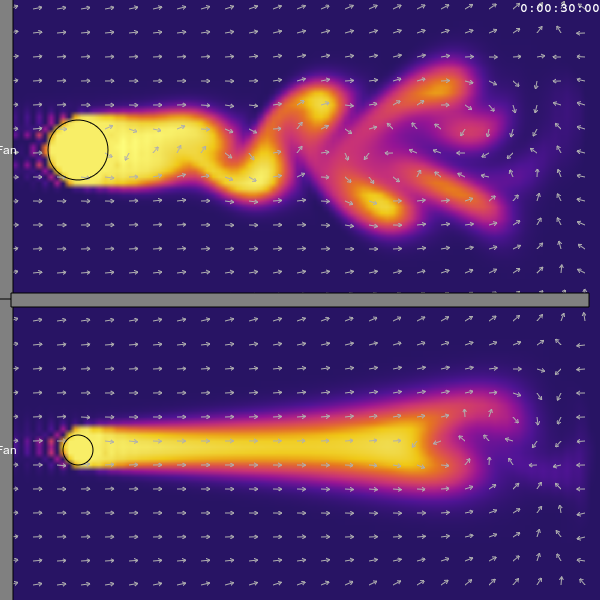
\includegraphics[width=.45\textwidth]{img/linSolvCPU5}
\caption{Symulacja przy użyciu metody Gaussa-Seidela na CPU, 
5 kroków relaksacji}
\label{fig:linSolvCPU5}

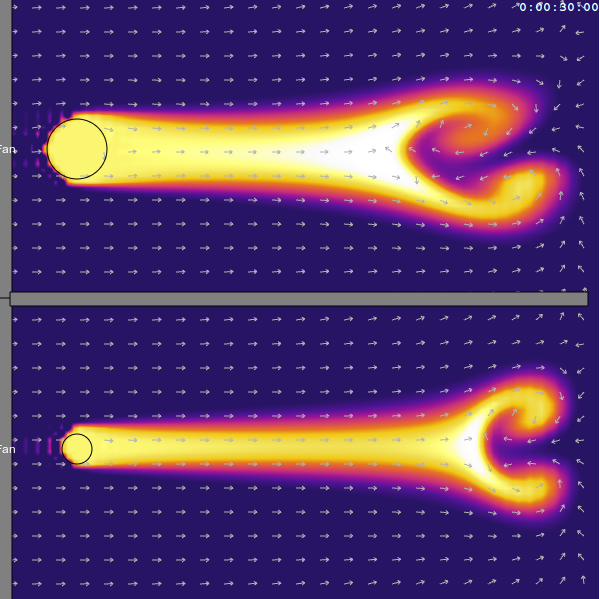
\includegraphics[width=.45\textwidth]{img/linSolvGPU5}
\caption{Symulacja przy użyciu metody Jacobiego na GPU, 
5 kroków relaksacji}
\label{fig:linSolvGPU5}

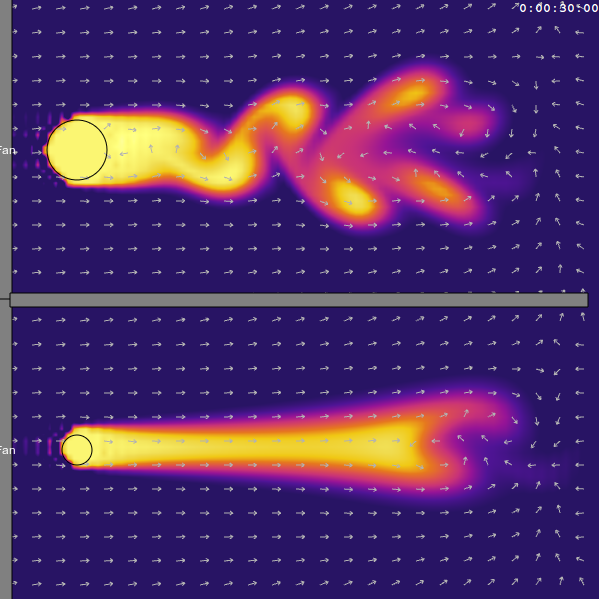
\includegraphics[width=.45\textwidth]{img/linSolvGPU10}
\caption{Symulacja przy użyciu metody Jacobiego na GPU, 
10 kroków relaksacji}
\label{fig:linSolvGPU10}

\end{figure}

Oczywiście zmiana algorytmu rozwiązywania równań liniowych niesie ze sobą
pewne konsekwencje. Inna jest konwergencja tych dwóch algorytmów. Metoda \ow
{Gaussa-Seidela} jest szybciej zbieżna niż metoda \ow{Jacobiego}. Efekty
symulacji dla różnej konfiguracji algorytmów rozwiązywania układów równań
liniowych prezentują rysunki \ref{fig:linSolvCPU5}, \ref{fig:linSolvGPU5} oraz
\ref{fig:linSolvGPU10}.

Na ww. rysunkach można zaobserwować wyraźne różnice w rezultatach symulacji. W
przypadku przedstawionej symulacji oczekiwanym wynikiem było powstane wiru
Kármána dla większej przeszkody. Przy implementacji równoległej metody
\ow{Jacobiego} widać, iż porządany efekt symulacji zostaje utracony. Dlatego
też należy wykonać więcej kroków relaksacji. Okazało się, że wartością
wystarczającą jest dziesięć. Wartość ta została ustalona empirycznie, tak aby
wyniki symulacji odpowiadały oczekiwaniom oraz były jak najbardziej zbliżone
do rezelutatów sekwencyjnych silików fizycznych. Jest to niezbędne, ponieważ
wersja równoległa aplikacji \en powinna być w pełni zgodnym i kompatybilnym
rozszerzeniem wersji podstawowej (sekwencyjnej, napisanej bez użycia
technologii \ow{WebGL}). Oczywiście wiąże się to ze spowolnieniem symulacji,
jednak w żadnym wypadku nie neguje opłacalności przeniesienia obliczeń na
kartę graficzną -- relaksacja na GPU jest wciąż dużo szybszych niż na CPU mimo
konieczności wykonania dwukrotnie większej liczby kroków.

Istnieją również implementacje algorytmu \ow{Gaussa-Seidela} na maszyny
równoległe. Nie są to dokładne kopie wersji sekwencyjnej, lecz imitują
obliczanie nowych wartości komórek na podstawie wartości z kroku relaksacji
poprzedniego i aktualnego. Doskonałe opracowanie zagadnień algorytmów
rozwiązujących układy równań liniowych na CPU oraz GPU, które okazało się
niezwykle przydatne podczas implementacji równoległych algorytmów dla \en,
zostało przygotowane przez G. Amadora oraz A. Gomesa \cite{LinSolvers}.
Niestety niskopoziomowa implementacja algorytmu \ow{Gaussa-Seidela} na GPU
wymaga wykonania dwóch procesów renderowania do tekstury dla jednego kroku
relaksacji -- powoduje to narzut czasowy, który w efekcie niweczy zysk z
szybszej konwergencji algorytmu.

\subsection{Podstawowy zarys implementacji}

Zgodnie z wnioskami sekcji \ref{subsec:srodPrzegInt}, ze względu na ograniczenia
środowiska przeglądarki internetowej, wymuszona została implementacja
niskopoziomowa przy użyciu technologii \ow{WebGL}. Opiera się ona na
programowaniu jednostek cieniujących karty graficznej, głównie wykorzystując
programy fragmentów (ang. fragment programs). Taka metoda przeprowadzania
obliczeń ogólnego przeznaczenia na karcie graficznej wymaga zrozumienia
podstawowych zagadnień związanych z programowaniem grafiki trójwymiarowej (por.
sekcja \ref{subsec:niskProgJedn}).

W przypadku implementacji \ow{Energy2D} podstawowy schemat przeprowadzania
obliczeń fizycznych na GPU z wykorzystaniem technologii \ow{WebGL} wygląda
następująco:

\begin{itemize}

\item Przygotowanie oraz kompilacja programów wierzchołków oraz fragmentów,
które zawierają implementację algorytmów silników fizycznych.

\item Przygotowanie tekstur, które przechowują dane symulacyjne. 

\item Przygotowanie danych geometrii płaszczyzny pokrywającej cały zakres
współrzędnych, które mieszczą się w obszarze renderowania.

\item Wykonywanie kolejnych kroków algorytmów fizycznych, co sprowadza się do:
	
	\begin{itemize}
	\item Renderowania wcześniej przygotowanej geometrii płaszczyzny przy użyciu
	wcześniej przygotowanych programów wierzchołków i fragmentów.

    \item Kopiowania danych z bufora ramki do wybranej tekstury przechowującej
	dane symulacji \footnote{Odbywa się to z użyciem obiektu bufora ramki (ang.
	FrameBuffer Object) z dołączoną do niego teksturą}.
	\end{itemize}

\end{itemize}

Poszczególne podpunkty w szerszym zakresie przybliżają sekcje od \ref{sec:progWierzFrag} do
\ref{sec:wykonNaGPU}.

\subsection{Programy wierzchołków oraz fragmentów}
\label{sec:progWierzFrag}

Właściwa implementacja algorytmów w programach wierzchołków i fragmentów
decyduje o poprawności oraz wydajności całej aplikacji. Bardzo często w
przypadku obliczeń ogólnego zastosowania na GPU, a także w przypadku
symulatora \ow{Energy2D}, większość pracy przypada na programy fragmentów.
Program wierzchołków zwykle sprowadza się do skopiowania wejściowych
współrzędnych wierzchołka i tekstury. Nie ma potrzeby jakiejkolwiek
modyfikacji geometrii renderowanej płaszczyzny. Dlatego też większość
programów wierzchołków w symulatorze Energy2D odpowiada poniższej
implementacji:

\begin{lstlisting}[language=GLSL, caption=Typowa implementacja programu
wierzchołków w symulatorze \ow{Energy2D} (język GLSL)]
attribute vec4 vertexPos;
attribute vec4 texCoord;

varying vec2 coord;
void main() {
  coord = texCoord;
  gl_Position = vertexPos;
}
\end{lstlisting}

Programy fragmentów, jako że wykonują właściwe obliczenia, nie są już tak
trywialne. Bardzo ważne jest właściwe określenie współrzędnych tekseli tekstury.
Posiadając siatkę symulacji o wymiarach NxN, należy ją zrzutować na zakres
domyślnych współrzędnych tekstury, które zawierają się w przedziale [0, 1].
Jeżeli zrobi się to nieprawidłowo, trudno będzie wykryć taki błąd, gdyż
domyślnie tekstury interpolują wartości leżące pomiędzy rzeczywistymi danymi.
Może to prowadzić do nieoczekiwanych rezultatów, stąd niezwykle istotne jest
precyzyjne określanie współrzędnych. W tym celu, praktycznie każdy program
fragmentów zawierał wektor o nazwie \ow{grid} równy (1.0 / N, 1.0 / N), gdzie
NxN to wymiary siatki symulacyjnej. Dodając lub odejmując odpowiedni jego
komponent można uzyskać dokładną wartość komórki sąsiedniej. Warto też pamiętać
o fakcie, iż pierwsza kolumna tekseli nie ma współrzędnej X równej 0.0, lecz 0.5
/ N. To samo dotyczy pierwszego rzędu współrzędnej Y równej 0.5 / N. Błędne
założenie, iż te kolumny mają współrzędne 0.0 prowadzi do problemów przy
wymuszaniu warunków brzegowych podczas symulacji. Ostatecznie, typowy szkielet
programów fragmentów wygląda następująco:

\begin{lstlisting}[language=GLSL, caption=Szkielet implementacji programu
fragmentów w symulatorze \ow{Energy2D} (język GLSL)]
uniform sampler2D simulationData;
uniform vec2 grid;
varying vec2 coord;

vec4 F(vec4 data) {
  // Funkcja wykonująca właściwe obliczenia dla danego kroku symulacji.
  // ...
}

void main() {
  vec4 data = texture2D(simulationData, coord);
  // Instrukcja warunkowa sprawdzająca czy nie są przetwarzane brzegi siatki.
  if (coord.x > grid.x && coord.x < 1.0 - grid.x &&
      coord.y > grid.y && coord.y < 1.0 - grid.y) {
    data = F(data);
  }
  gl_FragColor = data;
}
\end{lstlisting}

Oczywiście program, który wymuszał warunki brzegowe posiadał odwrotny warunek
w liniach 13 oraz 14. Implementacja funkcji $F$ nie jest przytoczona, gdyż nie
da się wyróżnić jakiegoś ogólnego jej schematu czy wzoru. Można powiedzieć, że
przenosząc dany krok algorytmu do języka GLSL, funkcja $F$ stanowi
implementację ,,wewnętrznych'' instrukcji zagnieżdżonych pętli iterujących po
wszystkich komórkach symulacji.


\subsection{Organizacja danych w pamięci karty graficznej}
\label{sec:orgDanychWGPU}
Dane symulacji (takie jak np. macierz temperatury czy macierz prędkości płynu)
przechowywane są w dwuwymiarowych teksturach zmiennoprzecinkowych. Tego typu
tekstury nie wchodzą w skład podstawowej specyfikacji \ow{WebGL 1.0}
(\cite{WebGLSpec}). W związku z tym wymagane jest użycie rozszerzenia
\ow{OES\_texture\_float}, które jest dostępne na większości
współczesnych urządzeń ([TODO: wspomnieć o rozdziale z testami]).

Niezwykle ważną kwestią jest organizacja danych w teksturze. Jest sporo
możliwości ponieważ tekstura z zasady nie jest wierną kopią tablicy JavaScript,
a obiektem przystosowanym do przechowywania obrazów (posiada na przykład kanały
kolorów). Dlatego też można rozważyć kilka potencjalnych sposobów na
rozmieszczenie danych.

\begin{itemize}

\item Schemat 1 -- tekstury jednokanałowe (format ALPHA lub LUMINANCE), jedna
tekstura odpowiada jednej tablicy JavaScript. Dalej nazywany schematem
\textbf{A1} na potrzeby niniejszego opracowania.

\item Schemat 2 -- tekstury czterokanałowe (format RGBA), dane tylko w jednym
kanale, jedna tekstura odpowiada jednej tablicy JavaScript. Dalej nazywany
schematem \textbf{RGBA1} na potrzeby niniejszego opracowania.

\item Schemat 3 -- tekstury czterokanałowe (format RGBA), dane w każdym z
kanałów, jedna tekstura odpowiada czterem tablicom JavaScript. Dalej nazywany
schematem \textbf{RGBA4} na potrzeby niniejszego opracowania.

\item Schemat 4 -- tekstury czterokanałowe (format RGBA), dane w każdym z
kanałów, jedna tekstura odpowiada jednej tablicy JavaScript, rozmiar tekstury
zredukowany czterokrotnie, gdyż każdy kanał odpowiada jednej ćwiartce tablicy.
Dalej nazywany schematem \textbf{RGBA1/4} na potrzeby niniejszego opracowania.

\end{itemize}

Każdy z powyższych schematów został przetestowany podczas implementacji
symulatora \ow{Energy2D}. Wyniki testów wydajnościowych przedstawia wykres
\ref{fig:texPerf}.

\begin{figure}[!h]
\centering
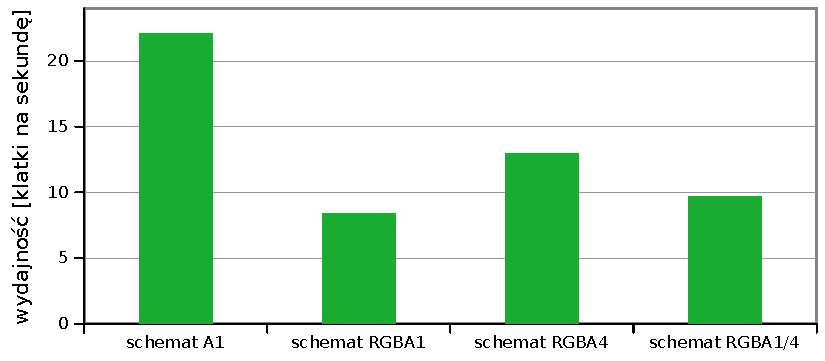
\includegraphics[width=.9\textwidth]{img/texPerf}
\caption{Wpływ organizacji danych w teksturach na wydajność symulacji 
\ow{Energy2D}}
\label{fig:texPerf}
\end{figure}

Rozwiązaniem optymalnym ze względu na wydajność oraz czytelność kodu wydaje się
schemat A1. Umożliwia on przeniesienie danych z tablic w relacji 1:1 do tekstur.
Do tego, każdy odczyt czy zapis do tekstury dotyczy tylko jednego kanału.
Niestety, na większości urządzeń nie ma możliwości dołączenia tekstury typu
ALPHA lub LUMINANCE do własnego obiektu bufora ramki (ang. FrameBuffer Object)
-- czyli renderowania do takiej tekstury \footnote{Testy zostały przeprowadzone
na systemie Linux (Ubuntu 12.04) i przeglądarce Google Chrome w wersji 22, która
korzysta z natywnego sterownika \ow{OpenGL}. Natomiast na tej samej konfiguracji
sprzętowej, ale działającej pod kontrolą systemu Windows nie udałoby się
uruchomić aplikacji. Podobnie w przypadku równie popularnego systemu
operacyjnego OS X.}. Wyklucza to możliwość użycia tego rozwiązania mimo
oczywistych zalet. Być może w przyszłości rozwój specyfikacji \ow{WebGL} na to
pozwoli.

Warto tutaj nadmienić, że specyfikacja \ow{WebGL} (\cite{WebGLSpec}) nie
gwarantuje, iż jakikolwiek z formatów tekstur zmiennoprzecinkowych będzie
zaakceptowany jako cel renderowania. Programista powinien wykonać test, aby
sprawdzić czy maszyna użytkownika wspiera daną konfigurację. Można to zrobić w
następujący sposób:

\begin{lstlisting}[language=JavaScript, caption=Weryfikacja poprawności formatu
i typu tekstury używanej jako cel renderowania]
var gl 		= getWebGLContext(),
	texture = gl.createTexture(),
	fbo 	= gl.createFramebuffer();

if (!gl.getExtension('OES_texture_float')) {
	throw new Error("Rozszerzenie OES_texture_float niedostępne.");
}
gl.bindTexture(gl.TEXTURE_2D, texture);
gl.texImage2D(gl.TEXTURE_2D, 0, gl.RGBA, 128, 128, 0, gl.RGBA, gl.FLOAT, null);
gl.bindFramebuffer(gl.FRAMEBUFFER, fbo);
gl.framebufferTexture2D(gl.FRAMEBUFFER, gl.COLOR_ATTACHMENT0, gl.TEXTURE_2D, texture, 0);
if (gl.checkFramebufferStatus(gl.FRAMEBUFFER) !== gl.FRAMEBUFFER_COMPLETE) {
	throw new Error("Dana tekstura nie jest wspierana jako cel renderowania.");
}
\end{lstlisting}

W praktyce tekstury zmiennoprzecinkowe posiadające cztery kanały kolorów są
najczęściej akceptowanym formatem do którego można zapisywać dane podczas
renderowania. Dlatego też schematy organizacji danych RGBA1, RGBA4 oraz RGBA1/4
używają takiego formatu tekstury.

Schemat RGBA1 posiada te same zalety co A1 jeśli chodzi o organizacje i
czytelność kodu źródłowego, jednak w tym przypadku dochodzi do dużego narzutu
wydajności związanego z odczytem i zapisem tekstur. Przy każdej z tych operacji
karta graficzna musi odczytać cztery kanały, jednak praktycznie wykorzystywany
jest tylko jeden z nich. Operacje dostępu do pamięci są czasochłonne, dlatego
też taka organizacja danych nie jest korzystna ze względów wydajnościowych.

Rozwiązaniem tego problemu są schematy RGBA4 oraz RGBA1/4. Organizacja danych
wg. trzeciego schematu pozwala zredukować narzut związany z odczytem oraz
zapisem pod warunkiem dobrej organizacji danych w teksturach. Pomysł ten
obrazuje diagram \ref{fig:rgba4Tex}. 

\begin{figure}[!h]
\centering
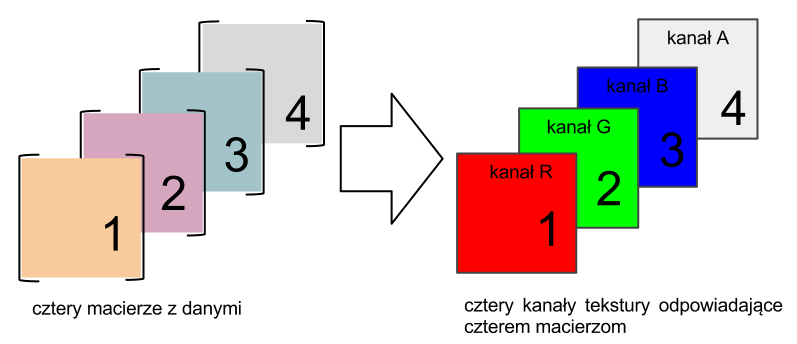
\includegraphics[width=.65\textwidth]{img/rgba4Tex}
\caption{Schemat organizacji danych z czterech macierzy w jednej teksturze}
\label{fig:rgba4Tex}
\end{figure}

Przy korzystnym ułożeniu danych jest możliwe praktycznie całkowite zredukowanie
narzutu związanego z odczytem wszystkich czterech kanałów tekstury, jednak w
praktyce jest to często niewykonalne. Przez korzystne rozmieszczenie danych
przyjmuje się takie ich ułożenie, żeby program jednostek cieniujących odczytując
teksturę faktycznie korzystał z danych zawartych w każdym z kanałów. Podobnie
przy zapisie, program renderujący powinien modyfikować wszystkie cztery kanały.
W przypadku symulatora \ow{Energy2D} udało się uzyskać taką organizację danych,
żeby odczyt był w znacznym stopniu zoptymalizowany, jednak podczas zapisu
modyfikowany był tylko jeden lub dwa kanały (kanał zawierający dane o
temperaturze lub kanały zawierające komponenty wektorów prędkości). Mimo nie do
końca optymalnego ułożenia kanałów, schemat RGBA4 okazał się wydajniejszy około
54\% od RGBA1.

\begin{figure}[!h]
\centering
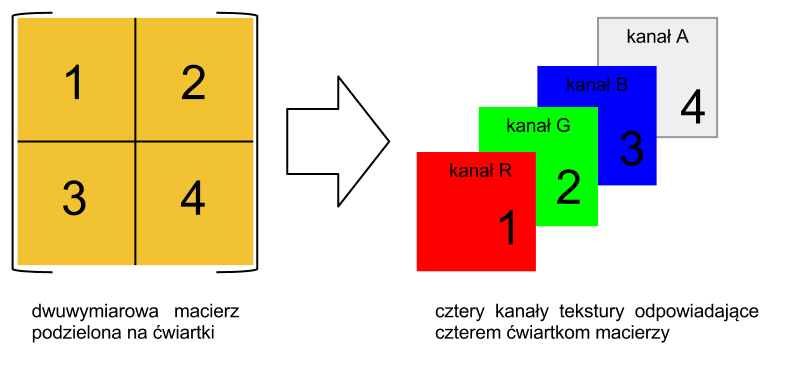
\includegraphics[width=.65\textwidth]{img/rgba14Tex}
\caption{Schemat organizacji danych macierzy NxN w teksturze (N/2)x(N/2)}
\label{fig:rgba14Tex}
\end{figure}

Ciekawą organizacją danych może wydawać się również pomysł przedstawiony w
schemacie RGBA1/4. Pozwala przechowywać tablicę JavaScript o wymiarach \ow{NxN}
w teksturze o wymiarach \ow{(N/2)x(N/2)}. Pomysł ten obrazuje diagram
\ref{fig:rgba14Tex}.

Taki układ danych teoretycznie posiada sporo zalet jak w przypadku użycia
tekstur jednokanałowych. Jednak znacznie zmniejsza on czytelność kodu i
komplikuje implementacje. Utrudnione zostaje przede wszystkim kontrolowanie
warunków brzegowych, programy jednostek cieniujących przetwarzają cztery pola
jednocześnie i stają się bardzo skomplikowane. W przypadku \ow{Energy2D}
komplikacje programów fragmentów były tak znaczne, że w efekcie odnotowano
bardzo słabe rezultaty pod względem wydajności. Symulacja okazała się być
wolniejsza około 34\% od symulacji korzystającej ze schematu RGBA4.

Dlatego też, ostatecznie w \ow{Energy2D} zastosowano schemat RGBA4. Zapewnia on
najlepszy kompromis pomiędzy dobrą wydajnością oraz wsparciem przez większość
dostępnych obecnie urządzeń.

\subsection{Geometria}

Podczas wykonywania obliczeń ogólnego przeznaczenia przy pomocy bezpośredniego
programowania jednostek cieniujących karty graficznej, niezbędne jest
stworzenie obiektu (a właściwie jego geometrii), który będzie renderowany. W
teorii może być to dowolna bryła. Jednak najczęściej pożądane jest, aby
program fragmentów wykonał się dla każdej komórki siatki symulacyjnej, którą
stanowi piksel tekstury. Można to osiągnąć renderując płaszczyznę, która
pokrywa całą dostępną przestrzeń renderowania.

Również w przypadku \en również wykorzystywany jest rendering takiej
płaszczyzny. Do przechowywania jej własności wykorzystane zostały bufory
wierzchołków (ang. vertex buffers) oraz indeksów (ang. index buffers)
znajdujące się w pamięci karty graficznej. Dzięki temu, podczas wielokrotnego
renderowania tej samej płaszczyzny, nie jest konieczne nieustanne przesyłanie
atrybutów wierzchołków do pamięci GPU.

W finalnej implementacji \en zostały przygotowane klasy pomocnicze
zarządzające geometrią oraz buforami. Jednak najprostszy sposób na stworzenie
płaszczyzny pokrywającej cały obszar renderowania oraz umieszczenie jej
atrybutów w pamięci karty graficznej zaprezentowany jest poniżej:

\begin{lstlisting}[language=JavaScript, caption=Definicja geometrii
płaszczyzny pokrywającej cały obszar renderowania]
var gl           = getWebGLContext(),
    vertexBuffer = gl.createBuffer(),
    indexBuffer  = gl.createBuffer(),
    vertexData,
    indexData;

// Współrzędne wierzchołków.
vertexData = new Float32Array([
    -1, -1, 
     1, -1,
    -1,  1,
     1,  1
]);
// Transfer do bufora wierzchołków.
gl.bindBuffer(gl.ARRAY_BUFFER, vertexBuffer);
gl.bufferData(gl.ARRAY_BUFFER, vertexData, gl.STATIC_DRAW);
// Indeksy trojkątów płaszczyzny.
indexData = new Uint16Array([
    0, 1, 2,
    2, 1, 3
]);
// Transfer do bufora indeksów.
gl.bindBuffer(gl.ELEMENT_ARRAY_BUFFER, indexBuffer);
gl.bufferData(gl.ELEMENT_ARRAY_BUFFER, indexData, gl.STATIC_DRAW);
\end{lstlisting}

\subsection{Wykonywanie kroków algorytmów na GPU}
\label{sec:wykonNaGPU}

Dysponując skompilowanymi programami wierzchołków oraz fragmentów, danymi
symulacji zapisanymi w teksturach dwuwymiarowych oraz niezbędną geometrią,
można przejść do faktycznej realizacji kroków algorytmów
zapisanych w programach jednostek cieniujących.

W przypadku technologii WebGL narzuca się schemat związany z techniką
renderowania do tekstury przy użyciu obiektu bufora ramki (ang. \emph{Frame
Buffer Object}). Związanie takiego obiektu z wybraną teksturą, a następnie
uaktywnienie przed właściwym renderowaniem, powoduje iż karta graficzna
automatycznie kopiuje zawartość bufora ramki do tekstury po zakończonym
renderowaniu.

Technika ta ma jednak kilka ograniczeń. Tekstura związana z obiektem bufora
ramki (czyli przeznaczona do zapisu) nie może być używana jednocześnie do
odczytu wartości. W związku z tym zawsze trzeba używać minimalnie jednej
tekstury tymczasowej. Następnie należy kopiować jej zawartość do tekstury
docelowej lub podmienić referencje. Oczywiście modyfikacja wyłącznie
referencji  jest znacznie efektywniejsza przez co i częściej stosowana.
Całościowo taki schemat nazywany jest ,,ping-pong rendering''.

Implementacja w języku \ow{JavaScript} przy użyciu technologi \ow{WebGL} nie
odbiega znacząco od implementacji w innych językach przy użyciu
,,tradycyjnego'' API OpenGL. Mark Harris zaprezentował najważniejsze aspekty
tej techniki w swoich artykułach opublikowanych w serii \emph{GPU Gems}
(\cite{GPUConcepts} oraz \cite{GPUFluid}).

	
\chapter{Ocena systemu}
	\section{Realizacja kluczowych wymagań}
	\section{Ocena dostępności aplikacji dla potencjalnych użytkowników}
		\subsection{Wpływ posiadanej konfiguracji sprzętowej i oprogramowania na symulator}
	\section{Modelowanie wybranych zjawisk fizycznych jako testy jakościowe symulatora}
	\section{Testy wydajnościowe}
		\subsection{Porównanie wydajności z symulatorem Energy2D opartym o platformę Java}
		\subsection{Zysk wydajności wynikający z przeniesienia obliczeń na GPU}
	\section{Wpływ optymalizacji i równoległości na jakość symulacji}
	\section{Podsumowanie oceny}
	
\chapter{Wnioski}
	\section{Podsumowanie}
	\section{Dalszy rozwój}

%\chapter{Wprowadzenie}
\label{cha:wprowadzenie}

Większość ludzi w swoich domach i pracy może korzystać z dorobku technologicznej
rewolucji, która miała miejsce w ostatnich latach. Jednak w niektórych
dziedzinach życia zmiany następują znacznie wolniej - jedną z nich jest
edukacja. Komputery i internet stały się dostępne w większości szkół, jednak
programy i metody nauczania często nie nadążają za postępem technologicznym, są
wciąż reliktem poprzedniej epoki. Uczniowie pracują na komputerach najnowszej
generacji, jednak zwykle wykorzystują tylko ułamki ich możliwości, nie mając
dostępu do narzędzi, które faktycznie mogłyby przyczynić się do lepszego
zrozumienia poruszanych na lekcjach zagadnień. Najczęściej komputer i internet
stają się po prostu źródłem łatwo dostępnej wiedzy czy też miejscem gdzie pewne
problemy można próbować rozwiązywać wspólnie. Jest to oczywiście prawidłowe i
wartościowe wykorzystanie nowoczesnej technologi, ale jednocześnie też dosyć
powierzchowne i niewyczerpujące jej pełnych możliwości. Problemy i wyzwania
stojące przed współczesną edukacją szerzej porusza Andrew A. Zucker
\cite{Zuc2009}.

Edukacja może skorzystać na technologicznej rewolucji w znacznie większym
stopniu - jednym z pomysłów są wirtualne laboratoria, które pozwolą uczniom
eksplorować wybrane zagadnienia w sposób interaktywny, szczególnie podczas
nauczania przedmiotów ścisłych i przyrodniczych, tak istotnych w dzisiejszych
czasach. Cyfryzacja powinna zmienić tradycyjne oblicze lekcji z podręcznikiem i
zeszytem na pracę przy narzędziach edukacyjnych nowej generacji, wykorzystując
powszechną dostępność nowoczesnych technologii. Takie aplikacje również
doskonale wpisują się w popularną ideę cyfrowych podręczników. Dosłowne
przeniesienie zawartości papierowych książek na ekrany komputerów nie wiązałoby
się ze znaczącymi zmianami - inny byłby tylko nośnik słów, wiedzy. Bez zmian
natomiast pozostałby sam proces i metody uczenia przez uczniów i studentów.
Jednak jeśli wirtualny podręcznik zostanie zintegrowany z interaktywnymi
aplikacjami, pozwoli to zupełnie zmienić oblicze nauki. Uczeń będzie miał
możliwość prawdziwej eksploracji zagadnień, eksperymentowania we własnym domu,
przed własnym komputerem, podczas codziennej nauki, która może zamienić się w
prawdziwą, wartościową i przede wszystkim rozwijającą przygodę.

Najlepszym pomysłem dla podręczników przyszłości wydaje się umiejscowienie ich w
internecie. Dzięki dystrybucji poprzez to medium można uzyskać niezwykle łatwy i
powszechny dostęp, jako że połączenie z internetem jest w dzisiejszych czasach
czymś w pełni osiągalnym. Internetowa dystrybucja niesie również mnóstwo
korzyści nie tylko dla użytkowników podręczników, ale także dla ich twórców -
wystarczy wymienić zalety takie jak łatwość aktualizacji i docierania do
odbiorców. W związku z tym, również narzędzia stanowiące interaktywne elementy
podręczników przyszłości powinny być przystosowane do działania w środowisku
przeglądarki internetowej. Jest to zadanie wymagające, jednak niedawny rozwój
technologii i standardów internetowych takich jak HTML5 oraz WebGL, jak również
gwałtowne zmiany w samych przeglądarkach internetowych, dają ogromne możliwości
w tej materii.

Wymienione pomysły nie są tylko planami na przyszłość - te zmiany już powoli
następują, cyfrowe podręczniki i wirtualne laboratoria są trakcie rozwoju. Jedną
z organizacji zajmujących się wprowadzaniem najnowszych osiągnięć techniki do
szkół jest \mbox{The Concord Consortium}.

\section{Cel pracy}
\label{sec:celPracy}

W wyniku współpracy ze wspomnianą organizacją \mbox{The Concord Consortium}
powstał wydajny symulator fizyczny prezentujący zjawisko przewodnictwa cieplnego
oraz dynamikę płynów działający w środowisku przeglądarki internetowej o nazwie
\emph{\mbox{Energy2D}}. Ta interaktywna aplikacja doskonale wpisuje się w
przedstawioną ideę wirtualnych podręczników i laboratoriów, umożliwiając
użytkownikom łatwiejsze zrozumienie praw fizyki, które rządzą transferem
energii.

Celem niniejszej pracy jest przedstawienie rozwiązań, które umożliwiły powstanie
symulatora, ze szczególnym naciskiem na technologię WebGL, której niestandardowe
i nowatorskie zastosowanie pozwoliło zrównoleglić obliczenia fizyczne i tym
samym osiągnąć znaczący wzrost wydajności.

\section{Organizacja dokumentu}
\label{sec:organizacjaDokumentu}

Dalsze rozdziały przedstawiają kolejno:

\begin{itemize} \item Przedstawienie możliwości symulatora \en, wprowadzenie
do problematyki symulacji dynamiki płynów i przewodnictwa cieplnego oraz
przegląd istniejących, podobnych rozwiązań.

\item Opis podstawowej implementacji aplikacji, ze szczególnym uwzględnieniem
zagadnień związanych z jej architekturą i wnioskami, które można rozszerzyć na
ogół złożonych systemów \ow{JavaScript}.

\item Prezentację kluczowych technik dzięki którym udało się zrównoleglić
silniki fizyczne symulatora \en przy pomocy technologii \ow{WebGL}.

\item Ocenę systemu, w szczególności testy jakościowe, wydajnościowe oraz
badanie jak konfiguracja sprzętowa użytkownika wpływa na odbiór i jakość
symulacji.

\item Podsumowanie, wnioski, oraz pomysły na dalszy rozwój aplikacji.
\end{itemize}

%\chapter{Przeniesienie obliczeń fizycznych na procesor karty graficznej}

Niniejszy rozdział prezentuje techniki zastosowane w celu przeniesienia głównych
obliczeń fizycznych na kartę graficzną w symulatorze \ow{Energy2D} będącym
przedmiotem tej pracy. Na początku opisane są tradycyjne podejścia do tego
problemu dla aplikacji działających w natywnym środowisku systemu operacyjnego
oraz ich odniesienie do środowiska oferowanego przez przeglądarki internetowe.
Następnie zaprezentowane zostały najważniejsze zagadnienia dotyczące
implementacji równoległych silników fizycznych \ow{Energy2D} działających na
procesorze karty graficznej. Informacje te mogą być szczególnie użyteczne przy
próbach podobnych optymalizacji innych aplikacji.

Dzięki przeniesieniu obliczeń fizycznych na GPU uzyskano istotny wzrost
wydajności. Dokładna analiza zysków ze zrównoleglenia symulacji jest przedstawiona
w rozdziale \ref{cha:ocena}.

\section{Typowe metody przenoszenia obliczeń na GPU, a przeglądarka internetowa}

Współczesna karty graficzne posiadają ogromną moc obliczeniową -- wielokrotnie
większą od centralnego procesora przy założeniu, że obliczenia da się wykonywać
w sposób równoległy. Pomysł aby przenieść część obliczeń ogólnego zastosowania
na kartę graficzną pojawił się wraz z dynamicznym rozwojem procesorów
graficznych. Szczególnie istotnym momentem było wprowadzenie programowalnych
jednostek cieniujących (specyfikacja \ow{DirectX 8}). Dalszy rozwój obliczeń
ogólnego zastosowania na kartach graficznych (ang. \emph{General-Purpose
Computing on Graphics Processing Units}, w skrócie GPGPU) miał miejsce wraz z
wprowadzeniem technologii, które ukryły złożoność dostępu do zasobów karty
graficznej i udostępniły interfejs wysokiego poziomu. Wiodącymi technologiami
tego typu są \ow{OpenCL} (rozwiązanie otwarte) oraz \ow{CUDA} (zamknięte
rozwiązanie firmy NVIDIA, działające wyłącznie na sprzęcie tego producenta).

Wspomniane powyżej technologie dotyczą oczywiście aplikacji pisanych w natywnym
środowisku systemu operacyjnego. Aby programować jednostki cieniujące wystarczy
podstawowy dostęp do standardowego interfejsu \ow{OpenGL} bądź \ow{Direct3D}.
Implementacje tych interfejsów można znaleźć dla prawie każdego współczesnego
języka programowania. Interfejsy wyższego poziomu (\ow{OpenCL}, \ow{CUDA})
również posiadają implementacje w różnych językach programowania, choć
najczęstszym środowiskiem ich działania są aplikacje napisane w C bądź C++.

Poniżej krótko przedstawione są sposoby przeprowadzania obliczeń ogólnego
zastosowania na kartach graficznych oraz ich związek ze specyficznym
środowiskiem przeglądarki internetowej.

\subsection{Niskopoziomowe programowanie jednostek cieniujących}
\label{subsec:niskProgJedn}

Jest to najstarsze podejście do przeprowadzania obliczeń ogólnego zastosowania
na procesorze karty graficznej. Programista w swoisty sposób ,,oszukuje'' kartę
graficzną, przeprowadzając renderowanie prostej geometrii wyłącznie w celu
uruchomienia własnych programów jednostek cieniujących, które wykonują
obliczenia często nie mające nic wspólnego z generowaniem obrazu.

W przypadku technologii \ow{WebGL}, która posłużyła do zaimplementowania
silników fizycznych \en, diagram potoku renderowania prezentuje rysunek
\ref{fig:WebGLPipeline}. Zielonym kolorem zostały oznaczone procesy, które są
programowalne. Są to dwa rodzaje programów jednostek cieniujących --
wierzchołków oraz fragmentów. Nie ma możliwości bezpośredniego sterowania
pozostałymi procesami. Odbywają się one automatycznie, ewentualnie możliwa jest
konfiguracja pewnych parametrów. Dlatego też cały algorytm przeznaczony do
zrównoleglenia musi zostać zapisany wyłącznie przy użyciu programów wierzchołków
oraz fragmentów. Ponadto dane powinny się znajdować w pamięci karty graficznej,
najczęściej w postaci dwuwymiarowych tekstur.

\begin{figure}[!h]
\centering
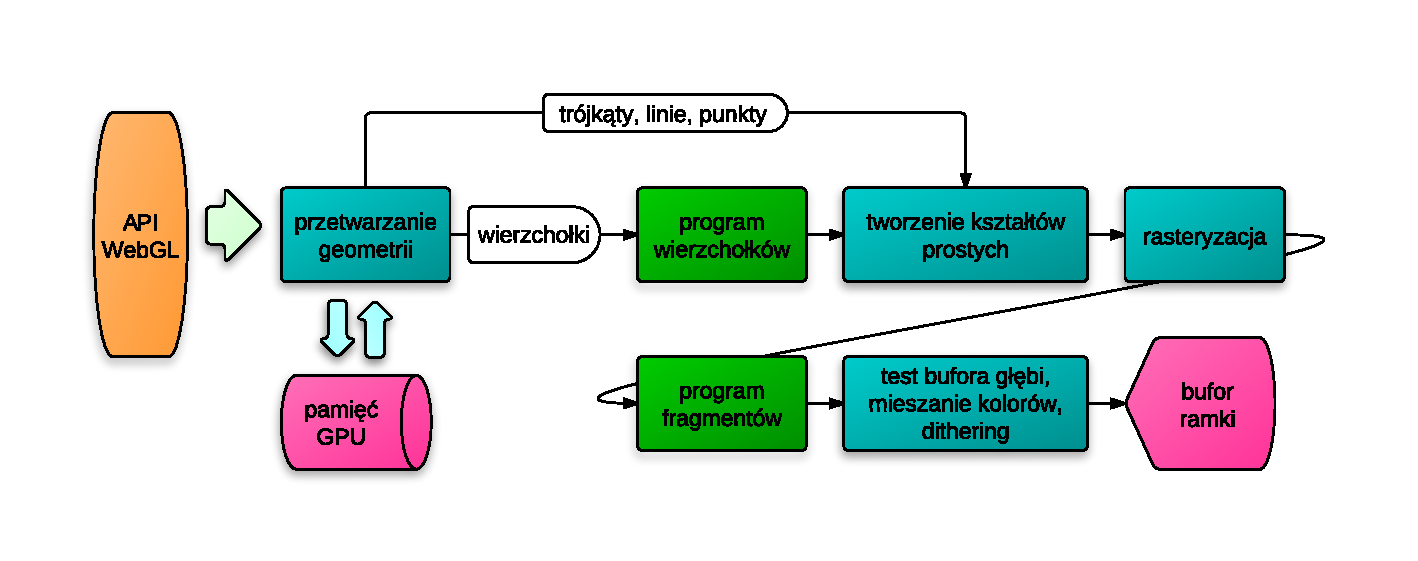
\includegraphics[width=\textwidth]{img/WebGLPipeline}
\caption{Diagram potoku renderowania \ow{WebGL} / \ow{OpenGL 3.x}}
\label{fig:WebGLPipeline}
\end{figure}

Takie podejście jednak jest wymagające i obarczone pewnymi problemami. Łatwo
popełnić błędy, wymagana jest też przynajmniej podstawowa wiedza o programowaniu
grafiki trójwymiarowej. Najważniejsze koncepcje niskopoziomowego programowania
jednostek cieniujących zostały doskonale przedstawione przez Marka Harrisa w
jednym z jego artykułów do popularnej serii \emph{GPU Gems} \cite{GPUConcepts}.

\subsection{Technologie wyższego poziomu}
\label{subsec:techWyzPoz}

Technologie, które przyczyniły się do gwałtownego wzrostu popularności obliczeń
na kartach graficznych to szczególnie \ow{OpenCL} oraz \ow{CUDA}.
Udostępniają  one znacznie wyższy poziom abstrakcji -- programista jest
zwolniony z obowiązku przyswojenia sobie niskopoziomowych mechanizmów rządzących
działaniem kart graficznych (choć ta wiedza pozwala tworzyć aplikacje
efektywniejsze). Udostępniony jest specjalny interfejs oraz składnia, co
znacznie ułatwia pracę, szczególnie programistom bez doświadczenia w pracy z
programowaniem grafiki trójwymiarowej.

\subsection{Możliwości w środowisku przeglądarki internetowej}
\label{subsec:srodPrzegInt}

Należy uściślić, że ,,środowisko przeglądarki internetowej'' to zbiór możliwości
nowoczesnych, wiodących przeglądarek internetowych, rozpowszechniony na tyle,
aby był dostępny dla większości użytkowników internetu. Równocześnie możliwości
te nie mogą wymagać instalowania żadnych dodatków i rozszerzeń, gdyż znacznie
ogranicza to ich dostępność. Jest to szczególnie istotne dla aplikacji
edukacyjnych, które wymagają łatwego i powszechnego dostępu.

Przeglądarka internetowa z założenia oferuje środowisko bardzo ograniczone,
przede wszystkim ze względów bezpieczeństwa. Jednak niedawno, wraz z nadejściem
standardu HTML5, został dodany podstawowy dostęp do zasobów karty graficznej.
Realizuje go technologia WebGL, która jest implementacją standardu \ow{OpenGL ES
2.0}. Tym samym pojawiła się możliwość programowania jednostek cieniujących kart
graficznych, a więc i przeprowadzania na nich obliczeń ogólnego zastosowania
(\ref{subsec:niskProgJedn}).

Technologie programowania kart graficznych wyższego poziomu
(\ref{subsec:techWyzPoz}) nie są (jeszcze) dostępne w przeglądarce internetowej.
Aktualnie trwają intensywne prace nad implementacją standardu OpenCL o roboczej
nazwie WebCL. Jednak technologia ta w aktualnym momencie jest na bardzo wczesnym
etapie rozwoju. Więcej informacji można znaleźć na stronie internetowej:
\url{http://www.khronos.org/webcl/}.

Dlatego też jedyną metodą na przeprowadzenie obliczeń ogólnego zastosowania na
procesorze karty graficznej w środowisku przeglądarki internetowej jest sposób
zaprezentowany w sekcji \ref{subsec:niskProgJedn}. Właśnie taka, niskopoziomowa
metoda została zastosowana dla silników fizycznych symulatora \ow{Energy2D}.
Opis najważniejszych zagadnień związanych z implementacją prezentuje następna
sekcja (\ref{sec:implSilFizWebGL}).

\section{Implementacji silników fizycznych Energy2D przy użyciu WebGL}
\label{sec:implSilFizWebGL}

Symulator \ow{Energy2D} składa się z dwóch kluczowych silników fizycznych -
przewodnictwa cieplnego oraz dynamiki płynów. Są one dokładnie przybliżone w
sekcji \ref{sec:silnikiFizyczne}. Oba te silniki są niezwykle wymagające
obliczeniowo. Dlatego też ich optymalizacja była zadaniem kluczowym, aby
stworzyć aplikację wartościową edukacyjnie. Zbyt wolny przebieg symulacji może
skutecznie zniechęcić większość potencjalnych użytkowników. Jednym z
podstawowych wymagań było, aby wirtualne laboratorium było aplikacją w pełni
interaktywną czyli również działającą jak najpłynniej.

Poniżej przedstawione są najważniejsze zagadnienia związanie z przeniesieniem
obliczeń fizycznych \ow{Energy2D} na kartę graficzną.

\subsection{Analiza algorytmów silników fizycznych pod kątem przetwarzania
równoległego}  

Wszystkie algorytmy rozwiązujące równania fizyczne w symulatorze \ow{Energy2D}
zostały poddane analizie pod kątem możliwości równoległego przetwarzania.
Zostały wyróżnione następujące kryteria, które algorytm musi spełniać, aby było
to możliwe:

\begin{itemize}

\item Możliwość reprezentowana danych w pamięci karty graficznej.

\item Niezależność wyniku algorytmu od sekwencji wykonywania obliczeń.

\end{itemize}

Jeżeli kryteria te są spełnione, powinna istnieć możliwość zaimplementowania
algorytmu w sposób równoległy. Oczywiście zmienia się strona techniczna, użyte
rozwiązania, język programowania oraz techniki, jednak sama koncepcja
algorytmu i główne kroki powinny pozostać bez większych zmian. Problem pojawia
się wtedy, gdy któryś z algorytmów nie spełnia jednego z tych kryteriów. W
takim przypadku konieczne są gruntowne modyfikacje lub rezygnacja z
implementacji takiego algorytmu.

Pierwszy warunek spełniają wszystkie algorytmy, jako że obliczenia są wykonywane
na prostokątnych siatkach symulacyjnych. Można je reprezentować w pamięci karty
graficznej przy użyciu dwuwymiarowych tekstur. Temat organizacji danych w
pamięci GPU oraz związane z tym problemy porusza sekcja \ref{sec:orgDanychWGPU}.

Drugi warunek nie został spełniony przez wszystkie zastosowane algorytmy.
Problematyczne okazały się metody rozwiązywania układów równań liniowych metodą
relaksacji \ow{Gaussa-Seidela} (por. \cite{GaussSeidel}). Podczas jednego
przebiegu przez wszystkie komórki macierzy, nowa wartość komórki $(i, j)$ jest
zależna od wartości komórek sąsiednich. Następnie komórka macierzy jest
niezwłocznie aktualizowana. Powoduje to, iż przy sekwencyjnym przetwarzaniu
wszystkich komórek, nowa wartość dla każdej komórki jest zależna od wartości
obliczonych zarówno w poprzednim kroku relaksacji jak i kroku aktualnym. W
sposób uproszczony schemat takiej relaksacji prezentuje algorytm
\ref{alg:GaussCPU}.

\begin{algorithm}[H]
  \caption{Relaksacja metodą Gaussa-Seidela na CPU}
  \label{alg:GaussCPU}
\begin{algorithmic}
\For {$0 \to relaxation\_steps$}
  \ForAll {$ \textrm{grid cells} $}
    \State $new\_val\gets f(x_{i,j}, x_{i+1,j}, x_{i-1,j}, x_{i,j+1}, x_{i,j-1})$
    \State $x_{i,j}\gets new\_val$
  \EndFor
\EndFor
\end{algorithmic}
\end{algorithm}

Niestety, przy obliczeniach równoległych nie można polegać na takiej zależności.
Każda komórka zostanie zaktualizowana na podstawie wartości komórek sąsiednich
wyłącznie z poprzedniego kroku relaksacji. Co więcej, ograniczeniem są też
kwestie czysto technologiczne - tekstury w których przechowywane są dane mogą
być podczas obliczeń wyłącznie przeznaczone do odczytu lub do zapisu. Tak więc
niemożliwy jest jednoczesny odczyt z danej tekstury oraz natychmiastowy zapis.

Problem ten został rozwiązany przez zmianę algorytmu rozwiązywania układów
równań liniowych na metodę relaksacji \ow{Jacobiego}. Główną różnicą jest moment
aktualizowania komórek siatki symulacji. W przeciwieństwie do metody \ow{Gaussa-
Seidela} nie następuje to natychmiast po obliczeniu nowej wartości dla danej
komórki, ale dopiero obliczeniu nowych wartości dla wszystkich komórek.
Uproszczony schemat tej relaksacji prezentuje algorytm \ref{alg:JacobiCPU}.

\begin{algorithm}[H]
  \caption{Relaksacja metodą Jacobiego na CPU}
  \label{alg:JacobiCPU}
\begin{algorithmic}
\For {$0 \to relaxation\_steps$}
  \ForAll {$ \textrm{grid cells} $}
    \State $temp_{i,j}\gets f(x_{i,j}, x_{i+1,j}, x_{i-1,j}, x_{i,j+1}, x_{i,j-1})$
  \EndFor
  \ForAll {$ \textrm{grid cells} $}
    \State $x_{i,j}\gets temp_{i,j}$
  \EndFor
\EndFor
\end{algorithmic}
\end{algorithm}

Taki algorytm można już przetworzyć na wersję równoległą. Macierze $x$ oraz
$temp$  zostają zamienione na odpowiednie tekstury. Również, w celach
wydajnościowych zawartość tekstur nie jest przepisywana tylko zamieniane są
ich referencje. Uproszczony schemat relaksacji metodą \ow{Jacobiego} na GPU
prezentuje algorytm \ref{alg:JacobiGPU}.

\begin{algorithm}[H]
  \caption{Relaksacja metodą Jacobiego na GPU}
  \label{alg:JacobiGPU}
\begin{algorithmic}
\For {$0 \to relaxation\_steps$}
  \ForAll {$ \textrm{grid cells} $} [IN PARALLEL]
    \State $temp_{i,j}\gets f(x_{i,j}, x_{i+1,j}, x_{i-1,j}, x_{i,j+1}, x_{i,j-1})$
  \EndFor
  \State swap $x$ with $temp$
\EndFor
\end{algorithmic}
\end{algorithm}

\begin{figure}[!p]
\centering

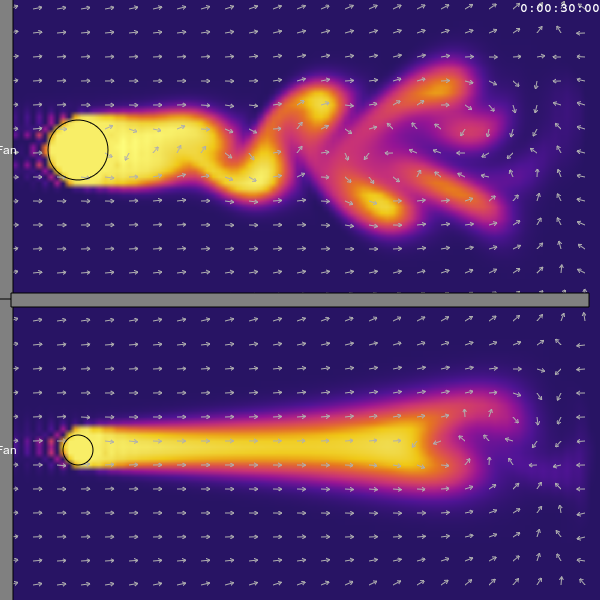
\includegraphics[width=.45\textwidth]{img/linSolvCPU5}
\caption{Symulacja przy użyciu metody Gaussa-Seidela na CPU, 
5 kroków relaksacji}
\label{fig:linSolvCPU5}

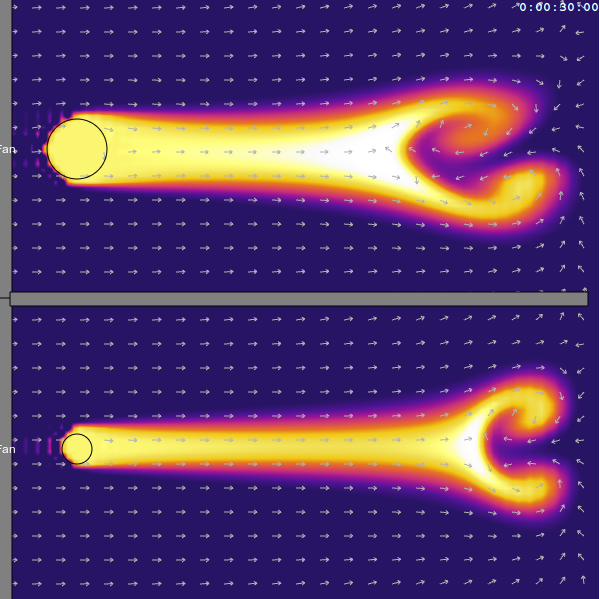
\includegraphics[width=.45\textwidth]{img/linSolvGPU5}
\caption{Symulacja przy użyciu metody Jacobiego na GPU, 
5 kroków relaksacji}
\label{fig:linSolvGPU5}

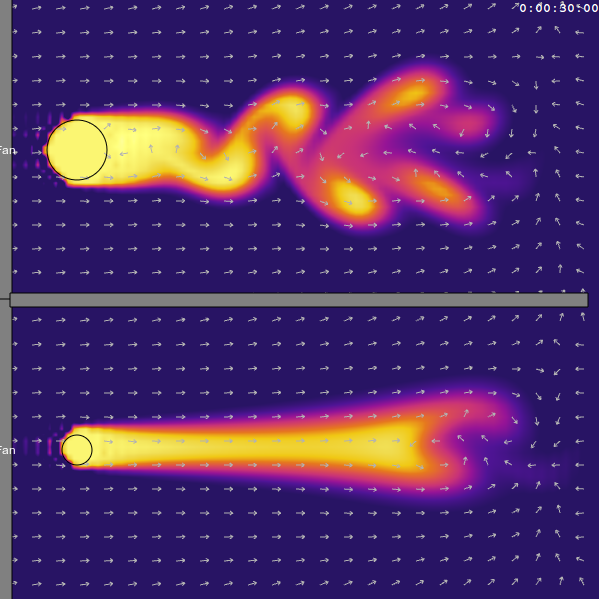
\includegraphics[width=.45\textwidth]{img/linSolvGPU10}
\caption{Symulacja przy użyciu metody Jacobiego na GPU, 
10 kroków relaksacji}
\label{fig:linSolvGPU10}

\end{figure}

Oczywiście zmiana algorytmu rozwiązywania równań liniowych niesie ze sobą
pewne konsekwencje. Inna jest konwergencja tych dwóch algorytmów. Metoda \ow
{Gaussa-Seidela} jest szybciej zbieżna niż metoda \ow{Jacobiego}. Efekty
symulacji dla różnej konfiguracji algorytmów rozwiązywania układów równań
liniowych prezentują rysunki \ref{fig:linSolvCPU5}, \ref{fig:linSolvGPU5} oraz
\ref{fig:linSolvGPU10}.

Na ww. rysunkach można zaobserwować wyraźne różnice w rezultatach symulacji. W
przypadku przedstawionej symulacji oczekiwanym wynikiem było powstane wiru
Kármána dla większej przeszkody. Przy implementacji równoległej metody
\ow{Jacobiego} widać, iż porządany efekt symulacji zostaje utracony. Dlatego
też należy wykonać więcej kroków relaksacji. Okazało się, że wartością
wystarczającą jest dziesięć. Wartość ta została ustalona empirycznie, tak aby
wyniki symulacji odpowiadały oczekiwaniom oraz były jak najbardziej zbliżone
do rezelutatów sekwencyjnych silików fizycznych. Jest to niezbędne, ponieważ
wersja równoległa aplikacji \en powinna być w pełni zgodnym i kompatybilnym
rozszerzeniem wersji podstawowej (sekwencyjnej, napisanej bez użycia
technologii \ow{WebGL}). Oczywiście wiąże się to ze spowolnieniem symulacji,
jednak w żadnym wypadku nie neguje opłacalności przeniesienia obliczeń na
kartę graficzną -- relaksacja na GPU jest wciąż dużo szybszych niż na CPU mimo
konieczności wykonania dwukrotnie większej liczby kroków.

Istnieją również implementacje algorytmu \ow{Gaussa-Seidela} na maszyny
równoległe. Nie są to dokładne kopie wersji sekwencyjnej, lecz imitują
obliczanie nowych wartości komórek na podstawie wartości z kroku relaksacji
poprzedniego i aktualnego. Doskonałe opracowanie zagadnień algorytmów
rozwiązujących układy równań liniowych na CPU oraz GPU, które okazało się
niezwykle przydatne podczas implementacji równoległych algorytmów dla \en,
zostało przygotowane przez G. Amadora oraz A. Gomesa \cite{LinSolvers}.
Niestety niskopoziomowa implementacja algorytmu \ow{Gaussa-Seidela} na GPU
wymaga wykonania dwóch procesów renderowania do tekstury dla jednego kroku
relaksacji -- powoduje to narzut czasowy, który w efekcie niweczy zysk z
szybszej konwergencji algorytmu.

\subsection{Podstawowy zarys implementacji}

Zgodnie z wnioskami sekcji \ref{subsec:srodPrzegInt}, ze względu na ograniczenia
środowiska przeglądarki internetowej, wymuszona została implementacja
niskopoziomowa przy użyciu technologii \ow{WebGL}. Opiera się ona na
programowaniu jednostek cieniujących karty graficznej, głównie wykorzystując
programy fragmentów (ang. fragment programs). Taka metoda przeprowadzania
obliczeń ogólnego przeznaczenia na karcie graficznej wymaga zrozumienia
podstawowych zagadnień związanych z programowaniem grafiki trójwymiarowej (por.
sekcja \ref{subsec:niskProgJedn}).

W przypadku implementacji \ow{Energy2D} podstawowy schemat przeprowadzania
obliczeń fizycznych na GPU z wykorzystaniem technologii \ow{WebGL} wygląda
następująco:

\begin{itemize}

\item Przygotowanie oraz kompilacja programów wierzchołków oraz fragmentów,
które zawierają implementację algorytmów silników fizycznych.

\item Przygotowanie tekstur, które przechowują dane symulacyjne. 

\item Przygotowanie danych geometrii płaszczyzny pokrywającej cały zakres
współrzędnych, które mieszczą się w obszarze renderowania.

\item Wykonywanie kolejnych kroków algorytmów fizycznych, co sprowadza się do:
	
	\begin{itemize}
	\item Renderowania wcześniej przygotowanej geometrii płaszczyzny przy użyciu
	wcześniej przygotowanych programów wierzchołków i fragmentów.

    \item Kopiowania danych z bufora ramki do wybranej tekstury przechowującej
	dane symulacji \footnote{Odbywa się to z użyciem obiektu bufora ramki (ang.
	FrameBuffer Object) z dołączoną do niego teksturą}.
	\end{itemize}

\end{itemize}

Poszczególne podpunkty w szerszym zakresie przybliżają sekcje od \ref{sec:progWierzFrag} do
\ref{sec:wykonNaGPU}.

\subsection{Programy wierzchołków oraz fragmentów}
\label{sec:progWierzFrag}

Właściwa implementacja algorytmów w programach wierzchołków i fragmentów
decyduje o poprawności oraz wydajności całej aplikacji. Bardzo często w
przypadku obliczeń ogólnego zastosowania na GPU, a także w przypadku
symulatora \ow{Energy2D}, większość pracy przypada na programy fragmentów.
Program wierzchołków zwykle sprowadza się do skopiowania wejściowych
współrzędnych wierzchołka i tekstury. Nie ma potrzeby jakiejkolwiek
modyfikacji geometrii renderowanej płaszczyzny. Dlatego też większość
programów wierzchołków w symulatorze Energy2D odpowiada poniższej
implementacji:

\begin{lstlisting}[language=GLSL, caption=Typowa implementacja programu
wierzchołków w symulatorze \ow{Energy2D} (język GLSL)]
attribute vec4 vertexPos;
attribute vec4 texCoord;

varying vec2 coord;
void main() {
  coord = texCoord;
  gl_Position = vertexPos;
}
\end{lstlisting}

Programy fragmentów, jako że wykonują właściwe obliczenia, nie są już tak
trywialne. Bardzo ważne jest właściwe określenie współrzędnych tekseli tekstury.
Posiadając siatkę symulacji o wymiarach NxN, należy ją zrzutować na zakres
domyślnych współrzędnych tekstury, które zawierają się w przedziale [0, 1].
Jeżeli zrobi się to nieprawidłowo, trudno będzie wykryć taki błąd, gdyż
domyślnie tekstury interpolują wartości leżące pomiędzy rzeczywistymi danymi.
Może to prowadzić do nieoczekiwanych rezultatów, stąd niezwykle istotne jest
precyzyjne określanie współrzędnych. W tym celu, praktycznie każdy program
fragmentów zawierał wektor o nazwie \ow{grid} równy (1.0 / N, 1.0 / N), gdzie
NxN to wymiary siatki symulacyjnej. Dodając lub odejmując odpowiedni jego
komponent można uzyskać dokładną wartość komórki sąsiedniej. Warto też pamiętać
o fakcie, iż pierwsza kolumna tekseli nie ma współrzędnej X równej 0.0, lecz 0.5
/ N. To samo dotyczy pierwszego rzędu współrzędnej Y równej 0.5 / N. Błędne
założenie, iż te kolumny mają współrzędne 0.0 prowadzi do problemów przy
wymuszaniu warunków brzegowych podczas symulacji. Ostatecznie, typowy szkielet
programów fragmentów wygląda następująco:

\begin{lstlisting}[language=GLSL, caption=Szkielet implementacji programu
fragmentów w symulatorze \ow{Energy2D} (język GLSL)]
uniform sampler2D simulationData;
uniform vec2 grid;
varying vec2 coord;

vec4 F(vec4 data) {
  // Funkcja wykonująca właściwe obliczenia dla danego kroku symulacji.
  // ...
}

void main() {
  vec4 data = texture2D(simulationData, coord);
  // Instrukcja warunkowa sprawdzająca czy nie są przetwarzane brzegi siatki.
  if (coord.x > grid.x && coord.x < 1.0 - grid.x &&
      coord.y > grid.y && coord.y < 1.0 - grid.y) {
    data = F(data);
  }
  gl_FragColor = data;
}
\end{lstlisting}

Oczywiście program, który wymuszał warunki brzegowe posiadał odwrotny warunek
w liniach 13 oraz 14. Implementacja funkcji $F$ nie jest przytoczona, gdyż nie
da się wyróżnić jakiegoś ogólnego jej schematu czy wzoru. Można powiedzieć, że
przenosząc dany krok algorytmu do języka GLSL, funkcja $F$ stanowi
implementację ,,wewnętrznych'' instrukcji zagnieżdżonych pętli iterujących po
wszystkich komórkach symulacji.


\subsection{Organizacja danych w pamięci karty graficznej}
\label{sec:orgDanychWGPU}
Dane symulacji (takie jak np. macierz temperatury czy macierz prędkości płynu)
przechowywane są w dwuwymiarowych teksturach zmiennoprzecinkowych. Tego typu
tekstury nie wchodzą w skład podstawowej specyfikacji \ow{WebGL 1.0}
(\cite{WebGLSpec}). W związku z tym wymagane jest użycie rozszerzenia
\ow{OES\_texture\_float}, które jest dostępne na większości
współczesnych urządzeń ([TODO: wspomnieć o rozdziale z testami]).

Niezwykle ważną kwestią jest organizacja danych w teksturze. Jest sporo
możliwości ponieważ tekstura z zasady nie jest wierną kopią tablicy JavaScript,
a obiektem przystosowanym do przechowywania obrazów (posiada na przykład kanały
kolorów). Dlatego też można rozważyć kilka potencjalnych sposobów na
rozmieszczenie danych.

\begin{itemize}

\item Schemat 1 -- tekstury jednokanałowe (format ALPHA lub LUMINANCE), jedna
tekstura odpowiada jednej tablicy JavaScript. Dalej nazywany schematem
\textbf{A1} na potrzeby niniejszego opracowania.

\item Schemat 2 -- tekstury czterokanałowe (format RGBA), dane tylko w jednym
kanale, jedna tekstura odpowiada jednej tablicy JavaScript. Dalej nazywany
schematem \textbf{RGBA1} na potrzeby niniejszego opracowania.

\item Schemat 3 -- tekstury czterokanałowe (format RGBA), dane w każdym z
kanałów, jedna tekstura odpowiada czterem tablicom JavaScript. Dalej nazywany
schematem \textbf{RGBA4} na potrzeby niniejszego opracowania.

\item Schemat 4 -- tekstury czterokanałowe (format RGBA), dane w każdym z
kanałów, jedna tekstura odpowiada jednej tablicy JavaScript, rozmiar tekstury
zredukowany czterokrotnie, gdyż każdy kanał odpowiada jednej ćwiartce tablicy.
Dalej nazywany schematem \textbf{RGBA1/4} na potrzeby niniejszego opracowania.

\end{itemize}

Każdy z powyższych schematów został przetestowany podczas implementacji
symulatora \ow{Energy2D}. Wyniki testów wydajnościowych przedstawia wykres
\ref{fig:texPerf}.

\begin{figure}[!h]
\centering
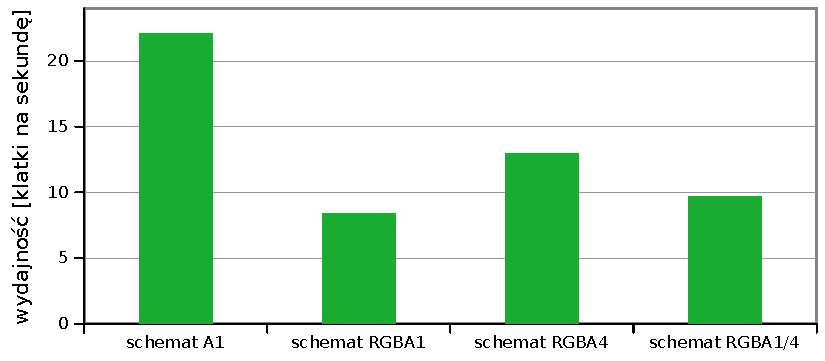
\includegraphics[width=.9\textwidth]{img/texPerf}
\caption{Wpływ organizacji danych w teksturach na wydajność symulacji 
\ow{Energy2D}}
\label{fig:texPerf}
\end{figure}

Rozwiązaniem optymalnym ze względu na wydajność oraz czytelność kodu wydaje się
schemat A1. Umożliwia on przeniesienie danych z tablic w relacji 1:1 do tekstur.
Do tego, każdy odczyt czy zapis do tekstury dotyczy tylko jednego kanału.
Niestety, na większości urządzeń nie ma możliwości dołączenia tekstury typu
ALPHA lub LUMINANCE do własnego obiektu bufora ramki (ang. FrameBuffer Object)
-- czyli renderowania do takiej tekstury \footnote{Testy zostały przeprowadzone
na systemie Linux (Ubuntu 12.04) i przeglądarce Google Chrome w wersji 22, która
korzysta z natywnego sterownika \ow{OpenGL}. Natomiast na tej samej konfiguracji
sprzętowej, ale działającej pod kontrolą systemu Windows nie udałoby się
uruchomić aplikacji. Podobnie w przypadku równie popularnego systemu
operacyjnego OS X.}. Wyklucza to możliwość użycia tego rozwiązania mimo
oczywistych zalet. Być może w przyszłości rozwój specyfikacji \ow{WebGL} na to
pozwoli.

Warto tutaj nadmienić, że specyfikacja \ow{WebGL} (\cite{WebGLSpec}) nie
gwarantuje, iż jakikolwiek z formatów tekstur zmiennoprzecinkowych będzie
zaakceptowany jako cel renderowania. Programista powinien wykonać test, aby
sprawdzić czy maszyna użytkownika wspiera daną konfigurację. Można to zrobić w
następujący sposób:

\begin{lstlisting}[language=JavaScript, caption=Weryfikacja poprawności formatu
i typu tekstury używanej jako cel renderowania]
var gl 		= getWebGLContext(),
	texture = gl.createTexture(),
	fbo 	= gl.createFramebuffer();

if (!gl.getExtension('OES_texture_float')) {
	throw new Error("Rozszerzenie OES_texture_float niedostępne.");
}
gl.bindTexture(gl.TEXTURE_2D, texture);
gl.texImage2D(gl.TEXTURE_2D, 0, gl.RGBA, 128, 128, 0, gl.RGBA, gl.FLOAT, null);
gl.bindFramebuffer(gl.FRAMEBUFFER, fbo);
gl.framebufferTexture2D(gl.FRAMEBUFFER, gl.COLOR_ATTACHMENT0, gl.TEXTURE_2D, texture, 0);
if (gl.checkFramebufferStatus(gl.FRAMEBUFFER) !== gl.FRAMEBUFFER_COMPLETE) {
	throw new Error("Dana tekstura nie jest wspierana jako cel renderowania.");
}
\end{lstlisting}

W praktyce tekstury zmiennoprzecinkowe posiadające cztery kanały kolorów są
najczęściej akceptowanym formatem do którego można zapisywać dane podczas
renderowania. Dlatego też schematy organizacji danych RGBA1, RGBA4 oraz RGBA1/4
używają takiego formatu tekstury.

Schemat RGBA1 posiada te same zalety co A1 jeśli chodzi o organizacje i
czytelność kodu źródłowego, jednak w tym przypadku dochodzi do dużego narzutu
wydajności związanego z odczytem i zapisem tekstur. Przy każdej z tych operacji
karta graficzna musi odczytać cztery kanały, jednak praktycznie wykorzystywany
jest tylko jeden z nich. Operacje dostępu do pamięci są czasochłonne, dlatego
też taka organizacja danych nie jest korzystna ze względów wydajnościowych.

Rozwiązaniem tego problemu są schematy RGBA4 oraz RGBA1/4. Organizacja danych
wg. trzeciego schematu pozwala zredukować narzut związany z odczytem oraz
zapisem pod warunkiem dobrej organizacji danych w teksturach. Pomysł ten
obrazuje diagram \ref{fig:rgba4Tex}. 

\begin{figure}[!h]
\centering
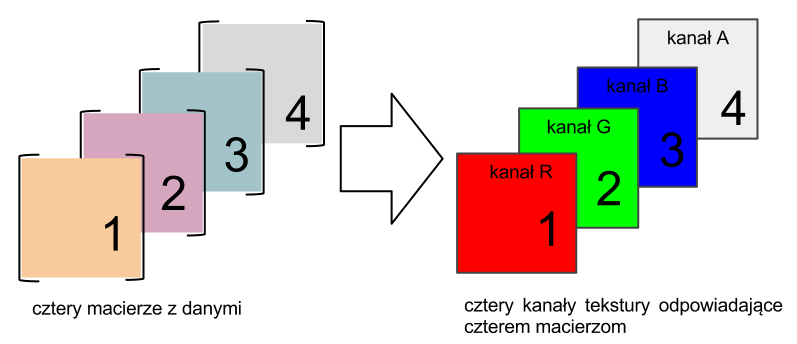
\includegraphics[width=.65\textwidth]{img/rgba4Tex}
\caption{Schemat organizacji danych z czterech macierzy w jednej teksturze}
\label{fig:rgba4Tex}
\end{figure}

Przy korzystnym ułożeniu danych jest możliwe praktycznie całkowite zredukowanie
narzutu związanego z odczytem wszystkich czterech kanałów tekstury, jednak w
praktyce jest to często niewykonalne. Przez korzystne rozmieszczenie danych
przyjmuje się takie ich ułożenie, żeby program jednostek cieniujących odczytując
teksturę faktycznie korzystał z danych zawartych w każdym z kanałów. Podobnie
przy zapisie, program renderujący powinien modyfikować wszystkie cztery kanały.
W przypadku symulatora \ow{Energy2D} udało się uzyskać taką organizację danych,
żeby odczyt był w znacznym stopniu zoptymalizowany, jednak podczas zapisu
modyfikowany był tylko jeden lub dwa kanały (kanał zawierający dane o
temperaturze lub kanały zawierające komponenty wektorów prędkości). Mimo nie do
końca optymalnego ułożenia kanałów, schemat RGBA4 okazał się wydajniejszy około
54\% od RGBA1.

\begin{figure}[!h]
\centering
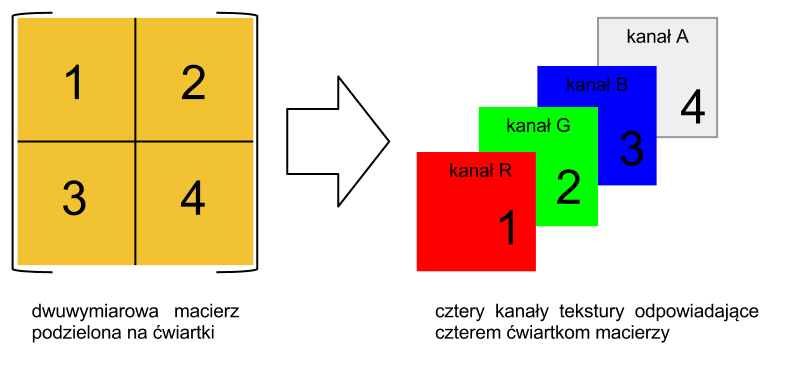
\includegraphics[width=.65\textwidth]{img/rgba14Tex}
\caption{Schemat organizacji danych macierzy NxN w teksturze (N/2)x(N/2)}
\label{fig:rgba14Tex}
\end{figure}

Ciekawą organizacją danych może wydawać się również pomysł przedstawiony w
schemacie RGBA1/4. Pozwala przechowywać tablicę JavaScript o wymiarach \ow{NxN}
w teksturze o wymiarach \ow{(N/2)x(N/2)}. Pomysł ten obrazuje diagram
\ref{fig:rgba14Tex}.

Taki układ danych teoretycznie posiada sporo zalet jak w przypadku użycia
tekstur jednokanałowych. Jednak znacznie zmniejsza on czytelność kodu i
komplikuje implementacje. Utrudnione zostaje przede wszystkim kontrolowanie
warunków brzegowych, programy jednostek cieniujących przetwarzają cztery pola
jednocześnie i stają się bardzo skomplikowane. W przypadku \ow{Energy2D}
komplikacje programów fragmentów były tak znaczne, że w efekcie odnotowano
bardzo słabe rezultaty pod względem wydajności. Symulacja okazała się być
wolniejsza około 34\% od symulacji korzystającej ze schematu RGBA4.

Dlatego też, ostatecznie w \ow{Energy2D} zastosowano schemat RGBA4. Zapewnia on
najlepszy kompromis pomiędzy dobrą wydajnością oraz wsparciem przez większość
dostępnych obecnie urządzeń.

\subsection{Geometria}

Podczas wykonywania obliczeń ogólnego przeznaczenia przy pomocy bezpośredniego
programowania jednostek cieniujących karty graficznej, niezbędne jest
stworzenie obiektu (a właściwie jego geometrii), który będzie renderowany. W
teorii może być to dowolna bryła. Jednak najczęściej pożądane jest, aby
program fragmentów wykonał się dla każdej komórki siatki symulacyjnej, którą
stanowi piksel tekstury. Można to osiągnąć renderując płaszczyznę, która
pokrywa całą dostępną przestrzeń renderowania.

Również w przypadku \en również wykorzystywany jest rendering takiej
płaszczyzny. Do przechowywania jej własności wykorzystane zostały bufory
wierzchołków (ang. vertex buffers) oraz indeksów (ang. index buffers)
znajdujące się w pamięci karty graficznej. Dzięki temu, podczas wielokrotnego
renderowania tej samej płaszczyzny, nie jest konieczne nieustanne przesyłanie
atrybutów wierzchołków do pamięci GPU.

W finalnej implementacji \en zostały przygotowane klasy pomocnicze
zarządzające geometrią oraz buforami. Jednak najprostszy sposób na stworzenie
płaszczyzny pokrywającej cały obszar renderowania oraz umieszczenie jej
atrybutów w pamięci karty graficznej zaprezentowany jest poniżej:

\begin{lstlisting}[language=JavaScript, caption=Definicja geometrii
płaszczyzny pokrywającej cały obszar renderowania]
var gl           = getWebGLContext(),
    vertexBuffer = gl.createBuffer(),
    indexBuffer  = gl.createBuffer(),
    vertexData,
    indexData;

// Współrzędne wierzchołków.
vertexData = new Float32Array([
    -1, -1, 
     1, -1,
    -1,  1,
     1,  1
]);
// Transfer do bufora wierzchołków.
gl.bindBuffer(gl.ARRAY_BUFFER, vertexBuffer);
gl.bufferData(gl.ARRAY_BUFFER, vertexData, gl.STATIC_DRAW);
// Indeksy trojkątów płaszczyzny.
indexData = new Uint16Array([
    0, 1, 2,
    2, 1, 3
]);
// Transfer do bufora indeksów.
gl.bindBuffer(gl.ELEMENT_ARRAY_BUFFER, indexBuffer);
gl.bufferData(gl.ELEMENT_ARRAY_BUFFER, indexData, gl.STATIC_DRAW);
\end{lstlisting}

\subsection{Wykonywanie kroków algorytmów na GPU}
\label{sec:wykonNaGPU}

Dysponując skompilowanymi programami wierzchołków oraz fragmentów, danymi
symulacji zapisanymi w teksturach dwuwymiarowych oraz niezbędną geometrią,
można przejść do faktycznej realizacji kroków algorytmów
zapisanych w programach jednostek cieniujących.

W przypadku technologii WebGL narzuca się schemat związany z techniką
renderowania do tekstury przy użyciu obiektu bufora ramki (ang. \emph{Frame
Buffer Object}). Związanie takiego obiektu z wybraną teksturą, a następnie
uaktywnienie przed właściwym renderowaniem, powoduje iż karta graficzna
automatycznie kopiuje zawartość bufora ramki do tekstury po zakończonym
renderowaniu.

Technika ta ma jednak kilka ograniczeń. Tekstura związana z obiektem bufora
ramki (czyli przeznaczona do zapisu) nie może być używana jednocześnie do
odczytu wartości. W związku z tym zawsze trzeba używać minimalnie jednej
tekstury tymczasowej. Następnie należy kopiować jej zawartość do tekstury
docelowej lub podmienić referencje. Oczywiście modyfikacja wyłącznie
referencji  jest znacznie efektywniejsza przez co i częściej stosowana.
Całościowo taki schemat nazywany jest ,,ping-pong rendering''.

Implementacja w języku \ow{JavaScript} przy użyciu technologi \ow{WebGL} nie
odbiega znacząco od implementacji w innych językach przy użyciu
,,tradycyjnego'' API OpenGL. Mark Harris zaprezentował najważniejsze aspekty
tej techniki w swoich artykułach opublikowanych w serii \emph{GPU Gems}
(\cite{GPUConcepts} oraz \cite{GPUFluid}).



% itd.
% \appendix
% \include{dodatekA}
% \include{dodatekB}
% itd.

\bibliographystyle{alpha}
\bibliography{bibliografia}
%\begin{thebibliography}{1}
%
%\bibitem{Dil00}
%A.~Diller.
%\newblock {\em LaTeX wiersz po wierszu}.
%\newblock Wydawnictwo Helion, Gliwice, 2000.
%
%\bibitem{Lam92}
%L.~Lamport.
%\newblock {\em LaTeX system przygotowywania dokumentów}.
%\newblock Wydawnictwo Ariel, Krakow, 1992.
%
%\bibitem{Alvis2011}
%M.~Szpyrka.
%\newblock {\em {On Line Alvis Manual}}.
%\newblock AGH University of Science and Technology, 2011.cccccc
%\newblock \\\texttt{http://fm.ia.agh.edu.pl/alvis:manual}.
%
%\end{thebibliography}

\end{document}
